\documentclass[withoutpreface,bwprint]{cumcmthesis}

\usepackage{float}
\usepackage{array}
\usepackage{makecell}
\usepackage{amsmath}
\usepackage{bm}
\usepackage{url}
\graphicspath{{../数据处理/}{figures/}}
\hypersetup{hidelinks}

\geometry{top=2.5cm,bottom=2.5cm,left=2.5cm,right=2.5cm}
\renewcommand*{\baselinestretch}{1.0}
\zihao{-4}\songti
\makeatletter
\renewcommand\section{\@startsection{section}{1}{\z@}%
  {-3.5ex \@plus -1ex \@minus -.2ex}%
  {2.3ex \@plus.2ex}%
  {\centering\normalfont\zihao{4}\heiti}}
\renewcommand\subsection{\@startsection{subsection}{2}{\z@}%
  {-3.25ex\@plus -1ex \@minus -.2ex}%
  {1.5ex \@plus .2ex}%
  {\normalfont\zihao{-4}\heiti}}
\renewcommand\subsubsection{\@startsection{subsubsection}{3}{\z@}%
  {-3.25ex\@plus -1ex \@minus -.2ex}%
  {1.5ex \@plus .2ex}%
  {\normalfont\zihao{-4}\heiti}}
\makeatother
\captionsetup[figure]{font={song,small},labelfont=bf}
\captionsetup[table]{font={song,small},labelfont=bf}

\newcommand{\paperTitle}{MIMAC 分子数据的活性筛选与结构风险评估}

\begin{document}
\setcounter{page}{1}
\pagenumbering{arabic}

\section{问题重述}

新药早期发现中，研究者往往需要从一批候选分子中判断哪些分子更值得优先进入下一轮实验。理想候选分子通常应具有较高的生物活性，但单纯追求高活性并不充分。若某分子周边存在大量结构相似但活性差异显著的分子，则说明该分子处于较陡峭的结构—活性关系区域，后续结构优化可能面临较高风险。因此，分子筛选过程需要同时考虑活性水平、结构稳定性和候选集合多样性。

本题给出了 MIMAC Dataset 的若干整理结果，包括分子二维流形坐标、生物活性得分、理化性质指标以及 KNN 近邻相似关系网络。要求围绕以下三个问题开展建模研究：

\begin{enumerate}
\item 在二维流形空间中对分子分布进行分区，识别高活性热点区域和普通区域，并比较不同区域在活性、相似关系或理化指标上的差异；
\item 建立分子对活性悬崖强度指标和单分子局部敏感度指标，结合第一问分区结果分析不同区域的稳定性，并判断高活性与高局部敏感度之间是否存在明显关联；
\item 在下一轮实验预算仅允许验证 8 个分子的条件下，综合考虑高活性、低局部敏感性和候选分子多样性，建立优选模型并给出推荐分子编号。


\end{enumerate}
\section{问题分析}

本题数据同时包含分子的空间嵌入、结构相似关系、活性响应以及若干理化性质，因此三个问题之间具有明显递进关系。第一问关注二维流形空间中高活性分子的空间富集现象；第二问关注相似结构之间活性突变所反映的局部风险；第三问则需要综合利用前两问得到的热点标签和局部敏感度指标，形成面向实验验证的候选分子集合。这一思路与结构—活性地貌分析中“先刻画局部 SAR 形态，再服务于分子筛选和优化”的思想一致\cite{ref:guha2012landscape}。

对于问题一，若仅使用传统聚类方法对二维坐标进行分区，得到的只是空间密度簇，不能直接体现高活性富集。已有研究在面波频散曲线自动拾取中提出基于能量密度的 E-DBSCAN 方法，表明在空间聚类中引入点属性权重有助于识别高能量富集区域\cite{ref:zhao2026edbscan}。受此启发，本文在 DBSCAN 思想基础上引入邻域活性密度，要求热点区域同时满足空间邻近性和活性富集性。

对于问题二，活性悬崖的本质是“结构相似但活性差异显著”。结构—活性地貌理论将此类局部不连续性视为 SAR 分析中的重要现象，并常用 SAS 图和 SALI 指数进行刻画\cite{ref:guha2012landscape,ref:guha2008sali}。附件 2 已给出分子之间的 KNN 相似网络及 Tanimoto 相似度，因此可直接在相似图边上计算分子对活性差异和 SALI 指数，再将分子对层面的悬崖强度汇总到单个分子层面，得到局部敏感度。

对于问题三，候选分子筛选不是单指标排序问题，而是固定规模集合的多目标组合优化问题。参考化合物选择研究已将候选集合构造表述为多目标设计问题，并利用遗传算法探索结构、理化性质和毒性响应等目标之间的 Pareto 权衡\cite{ref:ohto2026multiobjective}。若只选择活性最高的 8 个分子，可能导致局部敏感风险过高或分布过于集中；若过分强调多样性，又可能损失过多活性。因此本文采用 Pareto 多目标优化思想，在活性、风险和多样性之间进行权衡。


\section{模型假设}

为便于建模，本文作出如下假设：

\begin{enumerate}
\item 附件 1 中的二维流形坐标能够反映分子整体结构或性质上的相对邻近关系，可用于空间分区和多样性评价；
\item 附件 2 中的 KNN 图边表示分子之间具有较强局部相似关系，边权 \texttt{Tanimoto\_Similarity} 可作为结构相似性的度量；Tanimoto 相似度也是结构—活性地貌研究中常用的相似性度量\cite{ref:guha2012landscape}；
\item \texttt{Bioactivity\_Score} 能够表征分子的生物活性水平，分数越高表示活性越强；
\item 局部敏感度主要由相似邻域内的活性波动决定，KNN 图能够覆盖主要的局部结构变化关系；
\item 下一轮实验预算固定为 8 个分子，各候选分子实验成本近似相同。


\end{enumerate}
\section{符号说明}

\begin{table}[H]
\centering
\caption{主要符号说明}
\small
\resizebox{\textwidth}{!}{%
\begin{tabular}{ll}
\toprule
符号 & 含义 \\
\midrule
$D$ & 全部分子候选集合 \\
$N$ & 有效分子总数 \\
$i,j$ & 分子编号 \\
$X_i=(x_i,y_i)$ & 分子 $i$ 的二维流形坐标 \\
$A_i$ & 分子 $i$ 的生物活性得分 \\
$sim(i,j)$ & 分子 $i$ 与分子 $j$ 的 Tanimoto 结构相似度 \\
$N_\varepsilon(i)$ & 分子 $i$ 在二维流形空间中的 $\varepsilon$ 邻域 \\
$S_i$ & 分子 $i$ 的邻域活性总和 \\
$SALI_{ij}$ & 分子对 $(i,j)$ 的活性悬崖强度指数 \\
$LS_i$ & 分子 $i$ 的局部敏感度 \\
$S$ & 被选入下一轮实验的 8 分子集合 \\
\bottomrule
\end{tabular}%
}
\end{table}


\section{数据预处理}

本文主要使用两个附件数据。由于结构—活性地貌分析通常需要同时利用分子结构相似性与活性响应信息\cite{ref:guha2012landscape}，本文在预处理阶段保留二维坐标、活性得分、理化性质和 KNN 相似图四类信息：

\begin{enumerate}
\item \texttt{molecular\_interaction\_manifest.csv}：包含分子编号、SMILES、二维流形坐标 \texttt{Manifold\_X}、\texttt{Manifold\_Y}、生物活性得分 \texttt{Bioactivity\_Score} 以及若干理化性质指标；
\item \texttt{knn\_graph\_edges.csv}：包含 KNN 近邻相似图边表，其中 \texttt{Source} 和 \texttt{Target} 表示相似分子对，\texttt{Tanimoto\_Similarity} 表示结构相似程度。

\end{enumerate}
首先，对附件 1 中的数值型变量进行格式转换，选取二维流形坐标、生物活性得分和理化性质指标作为主要变量，并删除缺失 \texttt{Manifold\_X}、\texttt{Manifold\_Y} 或 \texttt{Bioactivity\_Score} 的样本。经处理后，共得到 325 个有效分子样本。

其次，读取附件 2 中的相似图边表，并将每条边对应的 Tanimoto 相似度作为结构相似性度量。经清洗后，共获得 1625 对有效相似分子对。若 KNN 图中同时存在 $i\to j$ 和 $j\to i$ 两条边，本文在局部敏感度计算中保留其作为有向近邻关系；在解释“分子对”数量时，该数量应理解为有效近邻边数量。


\section{问题一：二维流形空间分区与高活性热点识别}

\subsection{基于活性密度的 E-DBSCAN 模型}

传统 DBSCAN 方法主要依据空间密度识别聚类结构，但本题关注的是高活性分子在二维流形空间中的局部富集，而不是单纯的空间聚集。类似地，E-DBSCAN 方法通过将能量属性纳入邻域密度判定，提高了对高能量区域的识别能力\cite{ref:zhao2026edbscan}。因此本文构建基于活性密度的 E-DBSCAN 模型，将空间邻近性与邻域活性水平同时纳入热点识别。

对于第 $i$ 个分子，其二维流形坐标为

\[
X_i=(x_i,y_i),
\]

生物活性得分为

\[
A_i=Bioactivity\_Score_i.
\]

\subsubsection{邻域半径确定}

为了减少人为指定半径的主观性，本文采用第 8 近邻距离的中位数作为邻域半径。密度聚类类方法通常需要结合局部邻域尺度设定半径参数，而 E-DBSCAN 文献也指出不同数据集下聚类参数需要依据数据分布进行适配\cite{ref:zhao2026edbscan}。记 $d_{i,8}$ 为分子 $i$ 到其第 8 个最近邻的欧氏距离，则

\[
\varepsilon=\operatorname{median}(d_{i,8}).
\]

计算得到

\[
\varepsilon=0.2539.
\]

该半径能够反映样本在二维流形空间中的局部密度尺度。

\subsubsection{邻域活性密度}

定义分子 $i$ 的 $\varepsilon$ 邻域为

\[
N_{\varepsilon}(i)=\{j:\|X_j-X_i\|\leq \varepsilon\}.
\]

进一步定义分子 $i$ 的邻域活性总和为

\[
S_i=\sum_{j\in N_{\varepsilon}(i)}A_j.
\]

该指标不仅考虑中心分子自身活性，也反映其邻域内分子的整体活性水平。该处理与能量密度聚类中利用邻域能量总和判定核心点的思想相对应\cite{ref:zhao2026edbscan}，只是本文将物理能量替换为分子活性得分。本文取所有 $S_i$ 的 75\% 分位数作为核心点的最低邻域活性阈值：

\[
MinActivity=Q_{0.75}(S_i)=47.8175.
\]

同时，为避免低活性分子成为热点扩展起点，本文采用全体分子活性得分中位数作为活性初筛阈值：

\[
A_{threshold}=Q_{0.50}(A_i)=4.6015.
\]

当分子满足

\[
A_i\geq A_{threshold},\quad S_i\geq MinActivity
\]

时，将其视为热点核心候选点，并按照 DBSCAN 邻域扩展思想，将空间邻近且通过活性筛选的分子并入同一热点区域。未被归入热点区域的分子划分为普通区域。

\subsection{热点区域识别结果}

基于上述 E-DBSCAN 模型，本文共识别出 12 个高活性热点区域。其中热点区域分子 82 个，普通区域分子 243 个。结果说明，高活性分子并非完全随机散布于二维流形空间，而是在多个局部区域中呈现富集现象。

\begin{figure}[H]
\centering
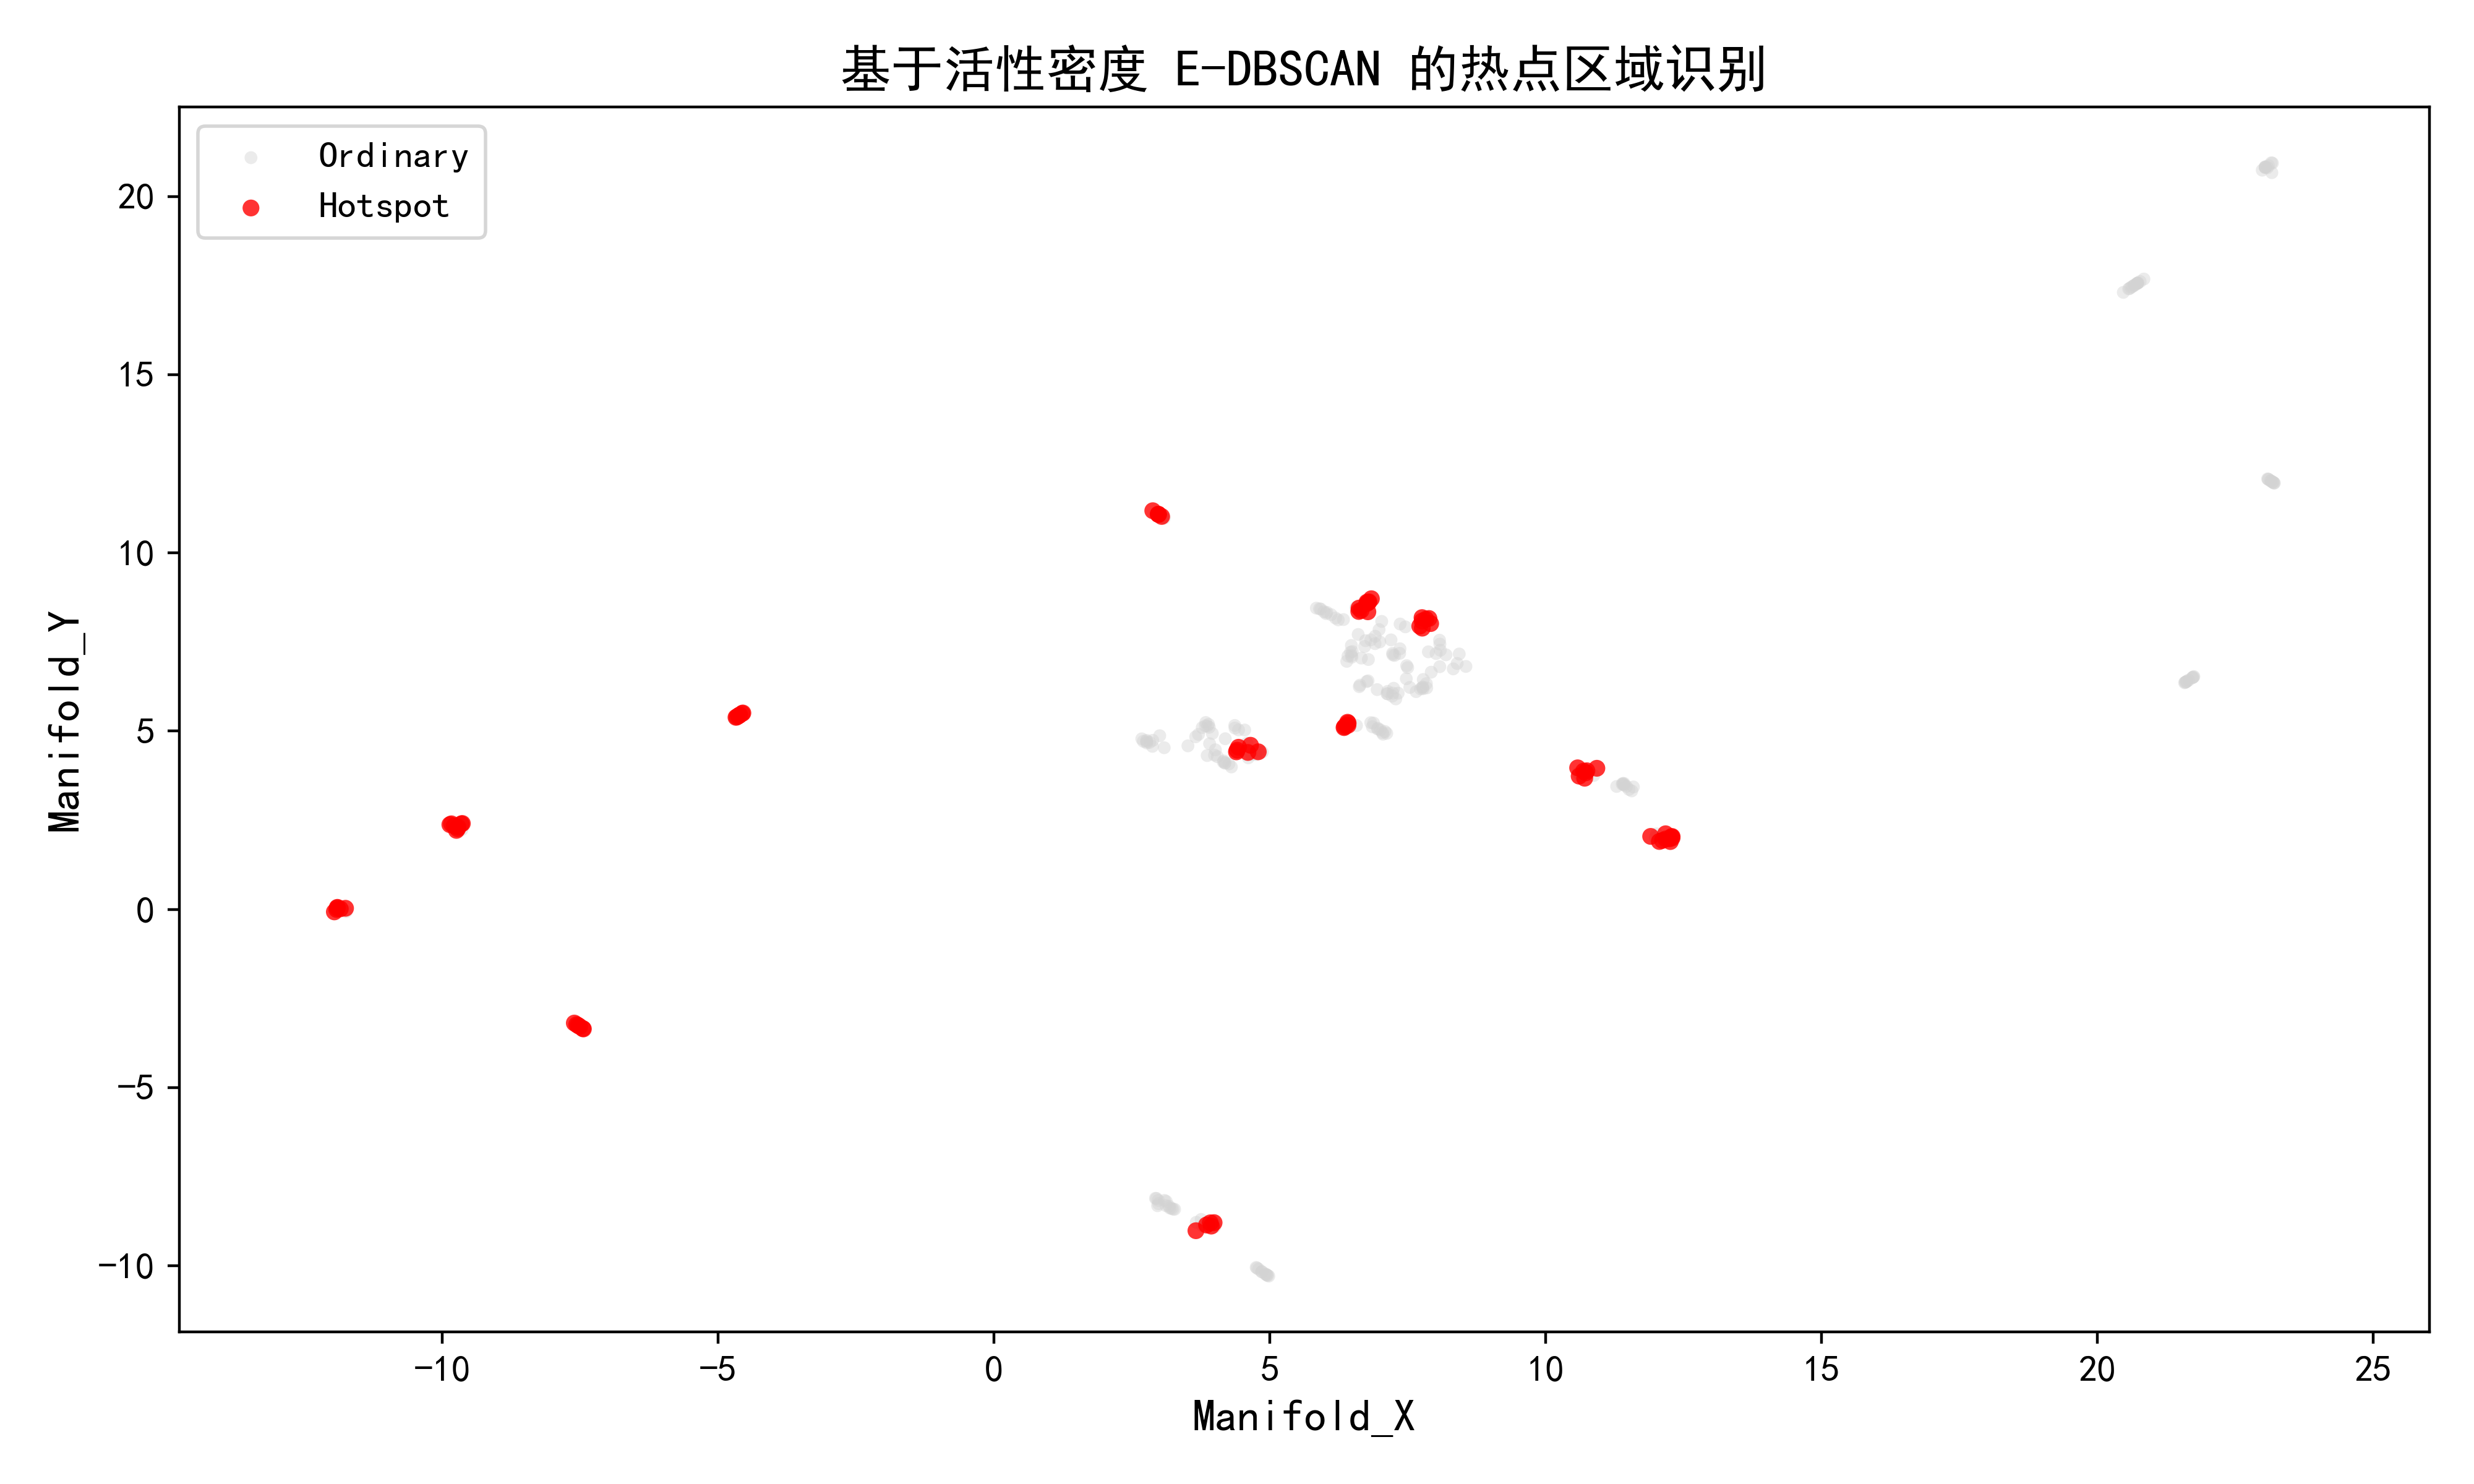
\includegraphics[width=0.82\textwidth]{问题1_热点区域识别结果.png}
\caption{基于活性密度 E-DBSCAN 的热点区域识别结果}
\end{figure}

进一步观察二维流形空间中的活性分布，高活性分子在部分局部区域内呈现较明显聚集趋势，为热点区域识别提供了直观依据。

\begin{figure}[H]
\centering
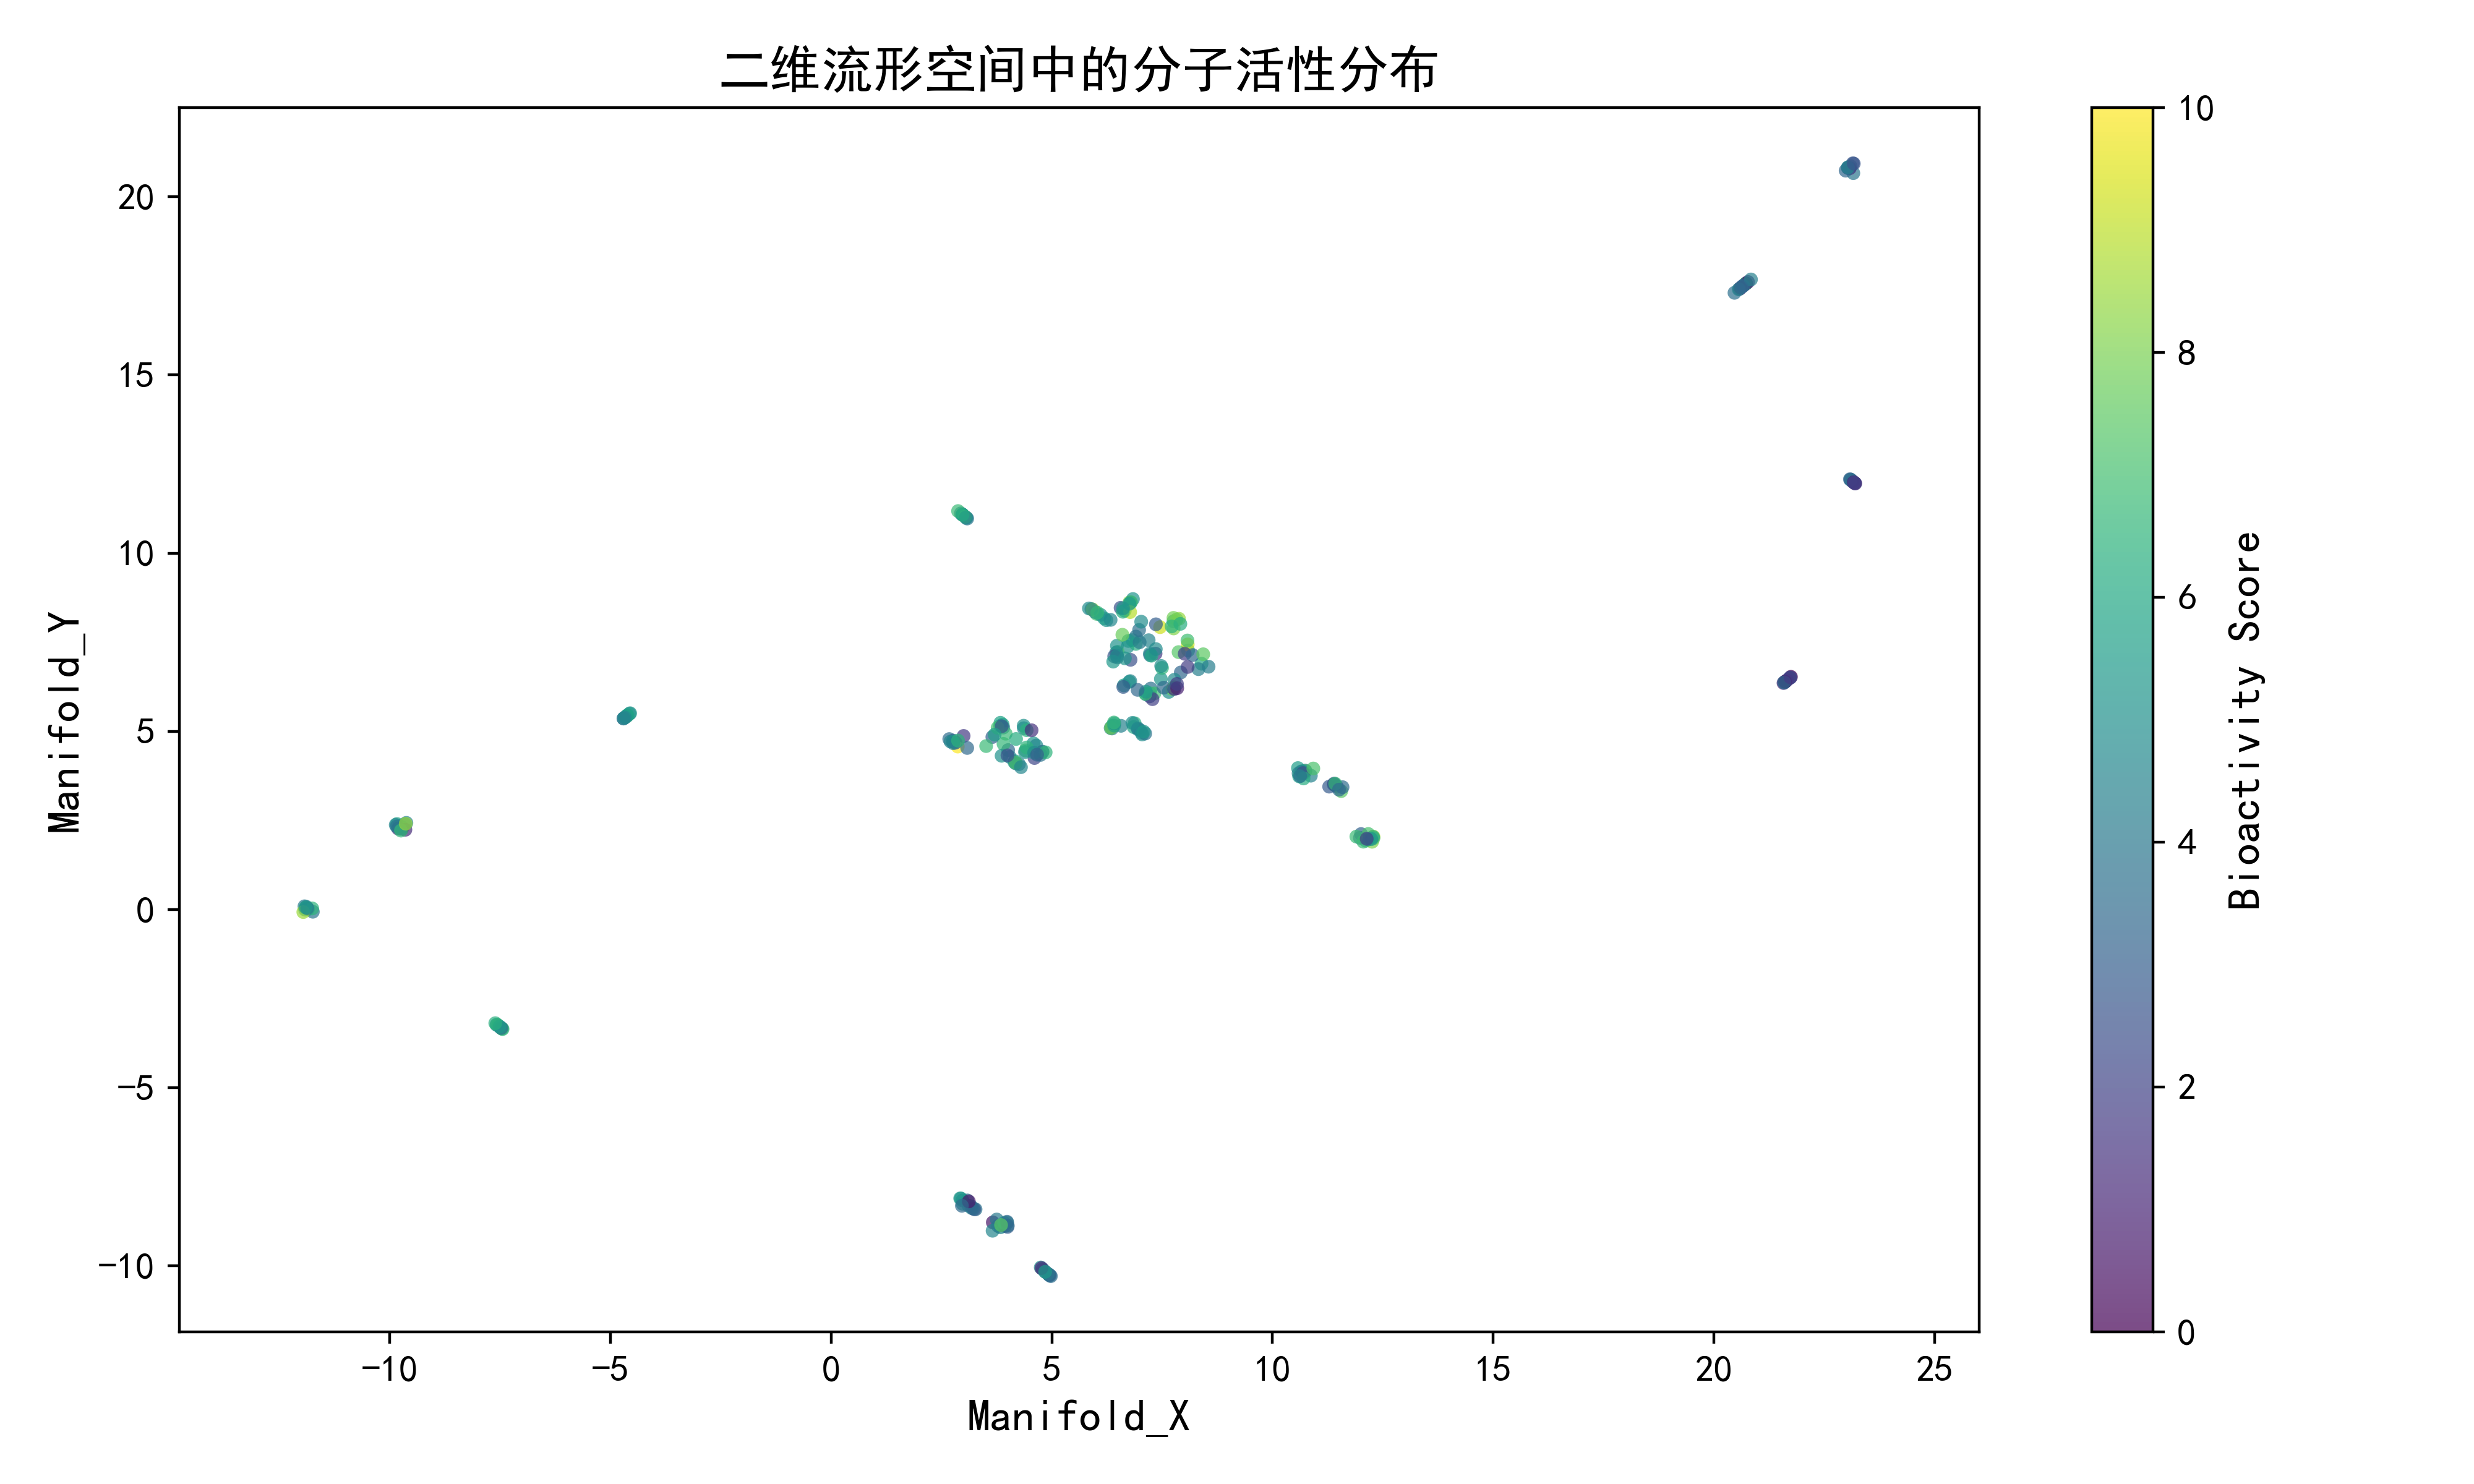
\includegraphics[width=0.82\textwidth]{问题1_二维流形空间分子活性分布.png}
\caption{二维流形空间中的分子活性分布}
\end{figure}

\subsection{热点区域与普通区域比较}

对热点区域与普通区域的生物活性进行统计比较，结果如下表所示。

\begin{table}[H]
\centering
\caption{热点区域与普通区域生物活性统计比较}
\small
\resizebox{\textwidth}{!}{%
\begin{tabular}{lllll}
\toprule
区域 & 分子数 & Bioactivity\_Score 均值 & Bioactivity\_Score 标准差 & Bioactivity\_Score 中位数 \\
\midrule
Hotspot & 82 & 6.2061 & 1.1376 & 6.1342 \\
Ordinary & 243 & 4.1201 & 1.7424 & 4.0342 \\
\bottomrule
\end{tabular}%
}
\end{table}

热点区域分子的平均活性得分为 6.2061，中位数为 6.1342；普通区域分子的平均活性得分为 4.1201，中位数为 4.0342。热点区域在均值和中位数上均明显高于普通区域，说明模型识别出的热点区域确实具有较高生物活性水平。

\begin{figure}[H]
\centering
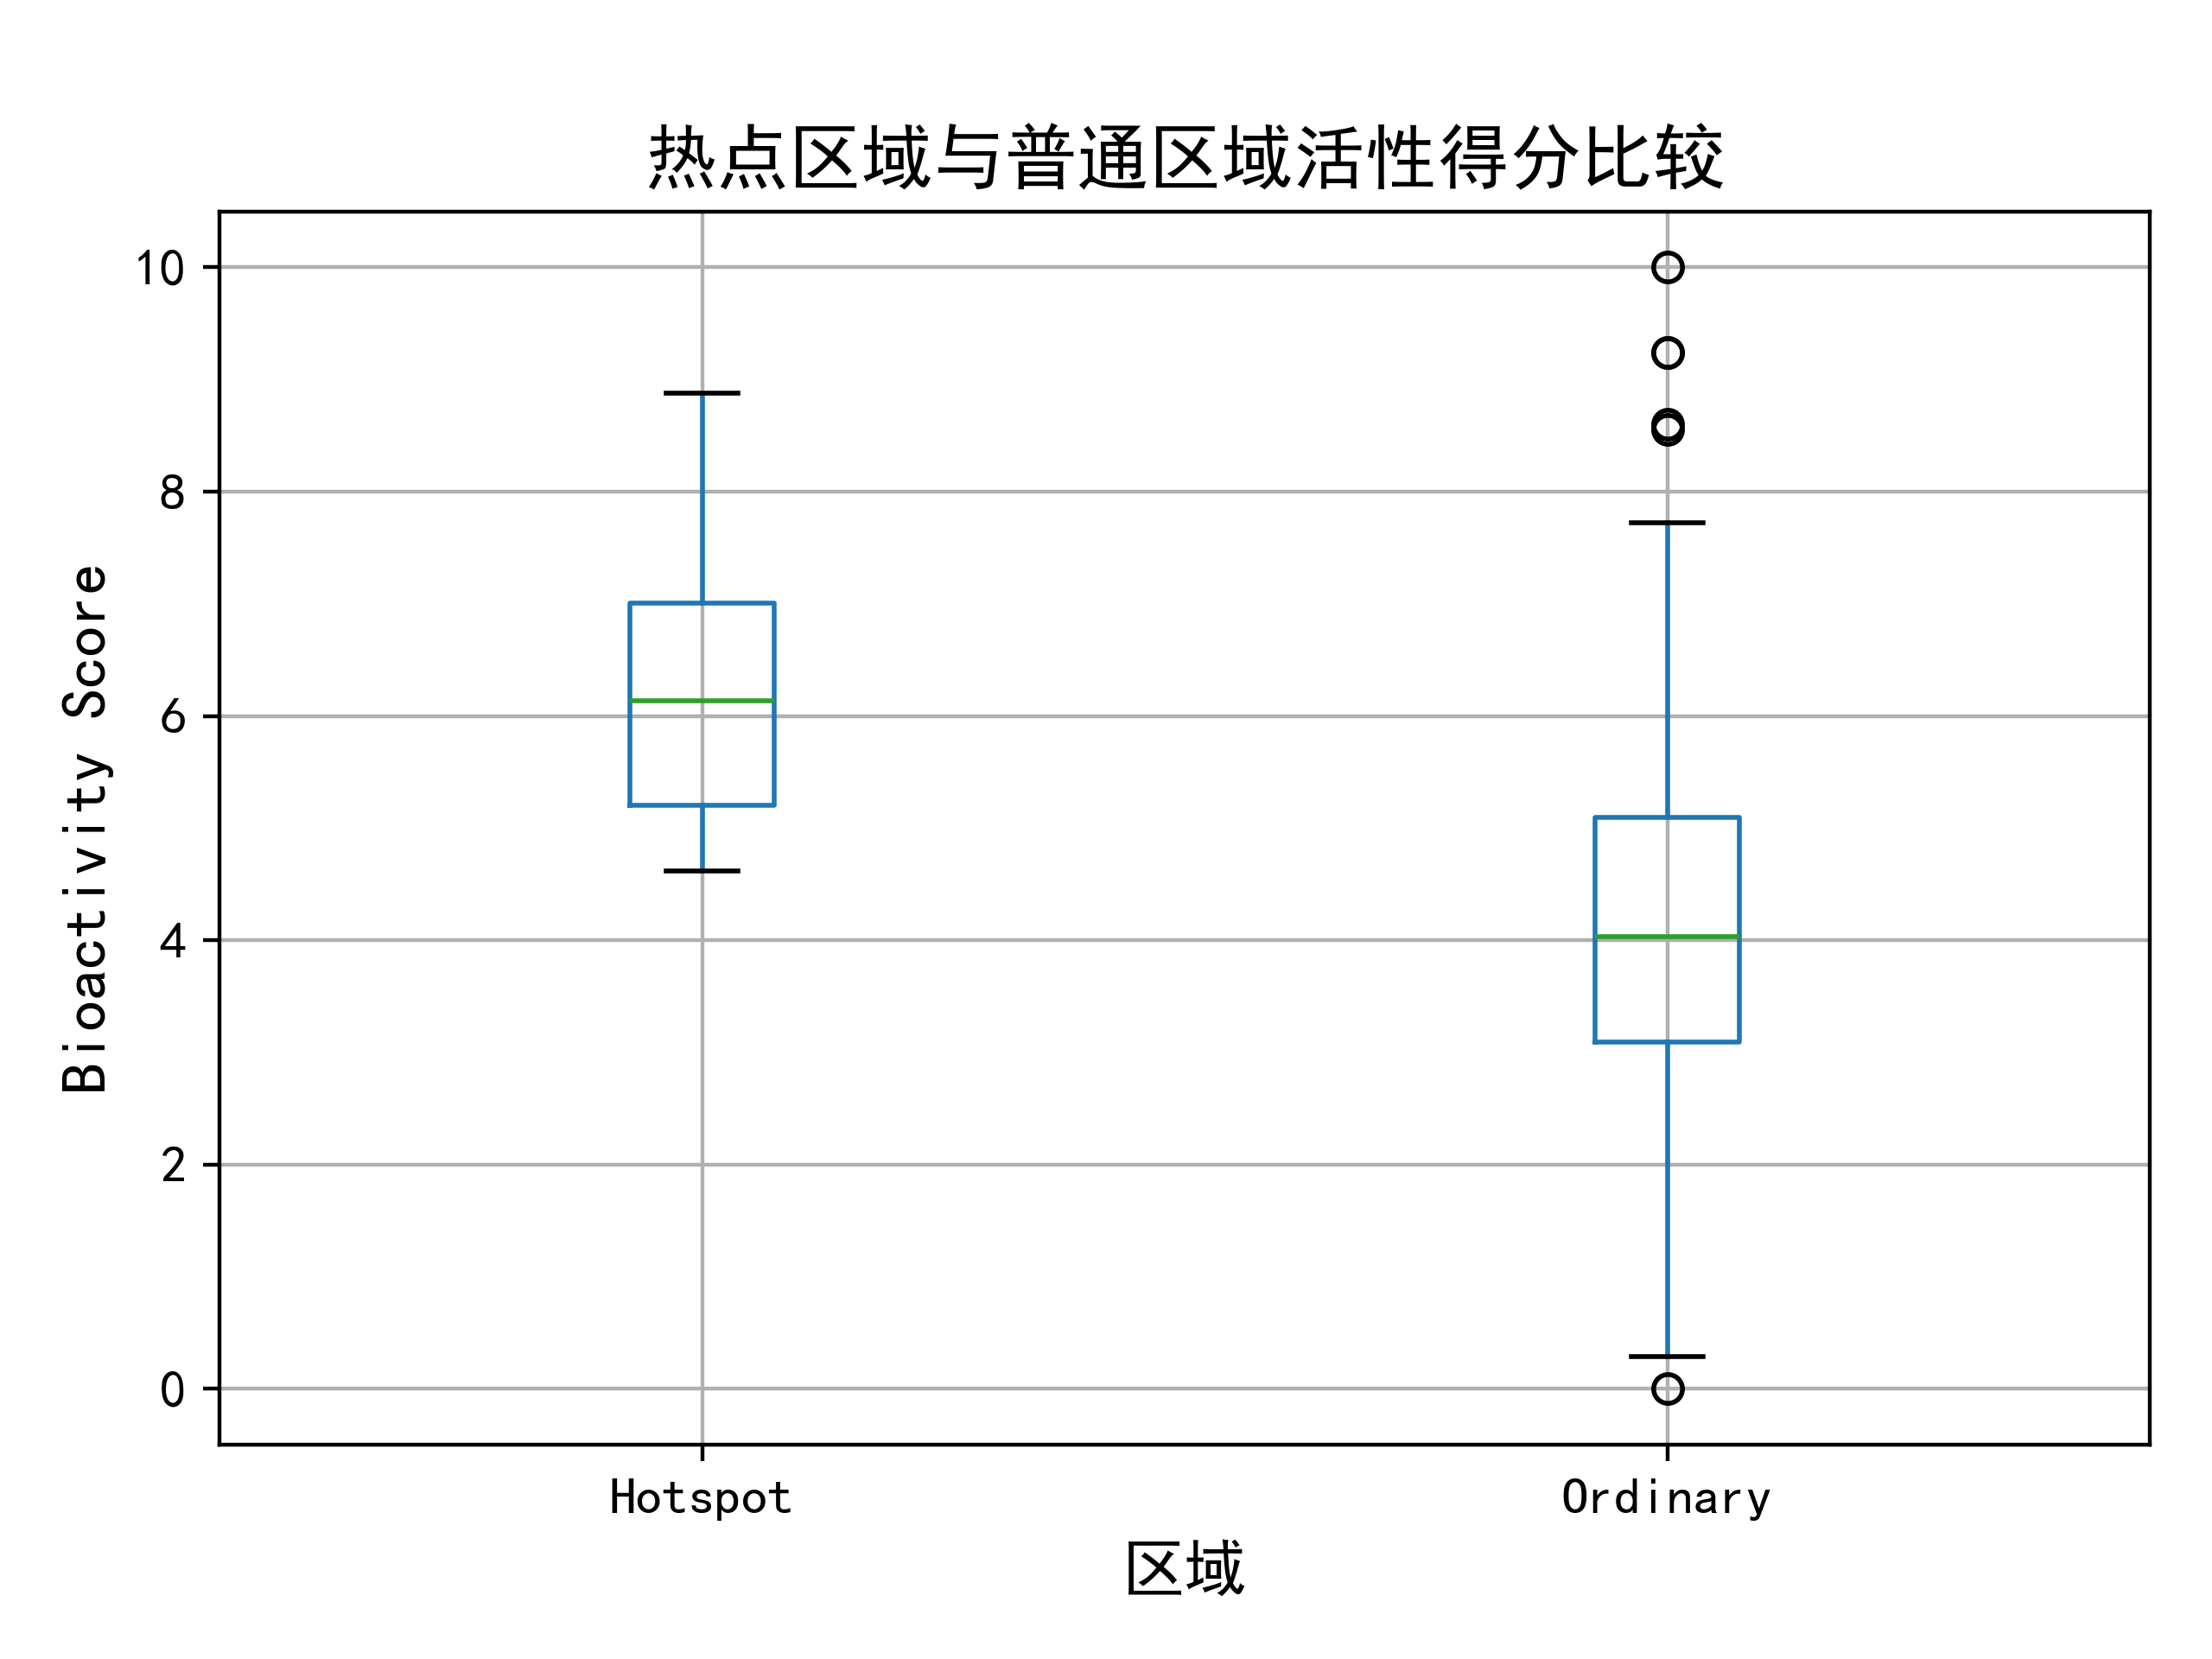
\includegraphics[width=0.82\textwidth]{问题1_热点区域与普通区域活性箱线图.png}
\caption{热点区域与普通区域生物活性得分比较}
\end{figure}

除生物活性外，热点区域在部分理化性质上也表现出差异。热点区域的 \texttt{MolWt} 均值为 159.0138，高于普通区域的 141.6394；热点区域的 \texttt{Bertz\_CT} 均值为 296.9286，高于普通区域的 200.8621。已有化合物选择研究也强调，结构覆盖与理化性质覆盖共同影响候选集合的代表性\cite{ref:ohto2026multiobjective}。这表明热点区域分子在分子量和结构复杂度方面整体偏高，可能与较高生物活性存在一定关联。

\subsection{各热点区域特征}

12 个热点区域在样本数量和平均活性方面存在差异，统计结果如下。

\begin{table}[H]
\centering
\caption{各热点区域活性统计结果}
\small
\resizebox{\textwidth}{!}{%
\begin{tabular}{llll}
\toprule
热点编号 & 分子数 & Bioactivity\_Score 均值 & Bioactivity\_Score 中位数 \\
\midrule
0 & 7 & 7.2112 & 7.8179 \\
1 & 5 & 6.3473 & 6.4354 \\
2 & 6 & 6.1572 & 5.9190 \\
3 & 10 & 6.7220 & 6.8154 \\
4 & 8 & 6.0862 & 5.8670 \\
5 & 7 & 6.1683 & 6.2158 \\
6 & 7 & 5.4815 & 5.2023 \\
7 & 6 & 5.9432 & 5.6727 \\
8 & 6 & 6.1629 & 6.4031 \\
9 & 6 & 5.8863 & 5.7437 \\
10 & 9 & 6.3414 & 6.1681 \\
11 & 5 & 5.4517 & 5.0648 \\
\bottomrule
\end{tabular}%
}
\end{table}

其中，热点区域 0 的平均活性最高，达到 7.2112；热点区域 3、1、10 的平均活性也相对较高。这表明二维流形空间中不同局部结构簇的活性富集程度并不完全相同。

\subsection{代表性分子分析}

为了说明分区结果的合理性，本文从热点区域中选取两类代表分子：一类为热点内最高活性分子，另一类为距离热点中心最近的中心代表分子；对于普通区域，则选取距离普通区域整体中心最近的分子作为代表。

\begin{table}[H]
\centering
\caption{不同区域代表性分子信息}
\small
\resizebox{\textwidth}{!}{%
\begin{tabular}{llllll}
\toprule
区域 & 热点编号 & 代表类型 & ID & SMILES & Bioactivity\_Score \\
\midrule
Hotspot & 0 & 热点内最高活性分子 & 101 & Nc1ccc2ccccc2c1 & 8.4053 \\
Hotspot & 0 & 热点中心代表分子 & 3 & Clc1ccc2ccccc2c1 & 5.6171 \\
Hotspot & 3 & 热点内最高活性分子 & 85 & C=CCC(C)c1ccccc1 & 8.6870 \\
Hotspot & 10 & 热点内最高活性分子 & 212 & C\#Cc1cccc(C(C)C)c1 & 8.8818 \\
Hotspot & 11 & 热点内最高活性分子 & 318 & C\#CC1CCCCC1 & 7.3994 \\
Ordinary & -1 & 普通区域代表分子 & 312 & O=C(O)Cc1cccc(O)c1 & 3.8368 \\
Ordinary & -1 & 普通区域代表分子 & 315 & O=C(O)Cc1cccc(F)c1 & 5.3872 \\
Ordinary & -1 & 普通区域代表分子 & 272 & Nc1cccc(CC(=O)O)c1 & 4.9750 \\
\bottomrule
\end{tabular}%
}
\end{table}

代表性分子结果表明，热点区域内确实存在较多高活性代表分子，而普通区域代表分子的活性整体较低或处于中等水平，从而进一步支持分区模型的合理性。


\section{问题二：活性悬崖强度与局部敏感度分析}

\subsection{分子对活性悬崖强度模型}

活性悬崖是指结构相似但生物活性存在显著差异的分子对，是结构—活性关系地貌中局部不连续区域的典型表现\cite{ref:guha2012landscape}。对于 KNN 图中的相似分子对 $(i,j)$，定义其活性差异为

\[
\Delta A_{ij}=|A_i-A_j|.
\]

为了在结构相似性与活性相似性平面中进行比较，本文定义活性相似度。该定义来源于结构—活性相似性图（SAS map）思想，可用于将平滑 SAR、活性悬崖和骨架跃迁等区域区分开来\cite{ref:guha2012landscape}：

\[
S_{Act}(i,j)=1-\frac{|A_i-A_j|}{A_{max}-A_{min}},
\]

其中 $A_{max}$ 和 $A_{min}$ 分别表示全体分子活性得分的最大值和最小值。活性差异越小，$S_{Act}$ 越接近 1。

进一步采用结构—活性地貌指数 SALI 刻画分子对悬崖强度，该指标可用于量化相似分子间活性突变程度\cite{ref:guha2008sali}：

\[
SALI_{ij}=\frac{|A_i-A_j|}{1-sim(i,j)}.
\]

当两个分子结构越相似时，$1-sim(i,j)$ 越小；若此时二者活性差异较大，则 $SALI_{ij}$ 会显著增大。因此，SALI 越大，说明该分子对越可能构成强活性悬崖。

本文采用分位数阈值识别活性悬崖。SAS 图和 SALI 网络在实际使用中通常需要结合数据集特点选取阈值，以突出最显著的局部不连续关系\cite{ref:guha2012landscape}。结构高相似阈值取

\[
sim_{cut}=Q_{0.75}(sim)=0.5789,
\]

活性低相似阈值取

\[
S_{Act,cut}=Q_{0.25}(S_{Act})=0.7348.
\]

若分子对满足

\[
sim(i,j)\geq sim_{cut},\quad S_{Act}(i,j)\leq S_{Act,cut},
\]

则定义为普通活性悬崖分子对。此外，以 SALI 的 95\% 分位数作为高强度活性悬崖阈值：

\[
SALI_{cut}=Q_{0.95}(SALI)=9.6204.
\]

当

\[
SALI_{ij}\geq SALI_{cut}
\]

时，将该分子对定义为高 SALI 活性悬崖分子对。

\subsection{活性悬崖识别结果}

对 1625 条有效近邻边进行分类，结果如下。

\begin{table}[H]
\centering
\caption{KNN 近邻边的活性悬崖类型统计}
\small
\resizebox{\textwidth}{!}{%
\begin{tabular}{lll}
\toprule
类型 & 数量 & 含义 \\
\midrule
Other & 1372 & 普通分子对 \\
Smooth SAR & 114 & 结构相似且活性相似的平滑结构—活性关系 \\
High SALI Cliff & 83 & SALI 最高的前 5\% 高强度活性悬崖 \\
Activity Cliff & 56 & 结构相似但活性差异较大的普通活性悬崖 \\
\bottomrule
\end{tabular}%
}
\end{table}

大多数相似分子对属于普通结构—活性关系，说明整体数据中相似结构之间的活性变化以相对平缓为主。但仍存在 83 对高 SALI 活性悬崖和 56 对普通活性悬崖，说明局部结构空间中存在一定数量的活性突变现象。

\begin{figure}[H]
\centering
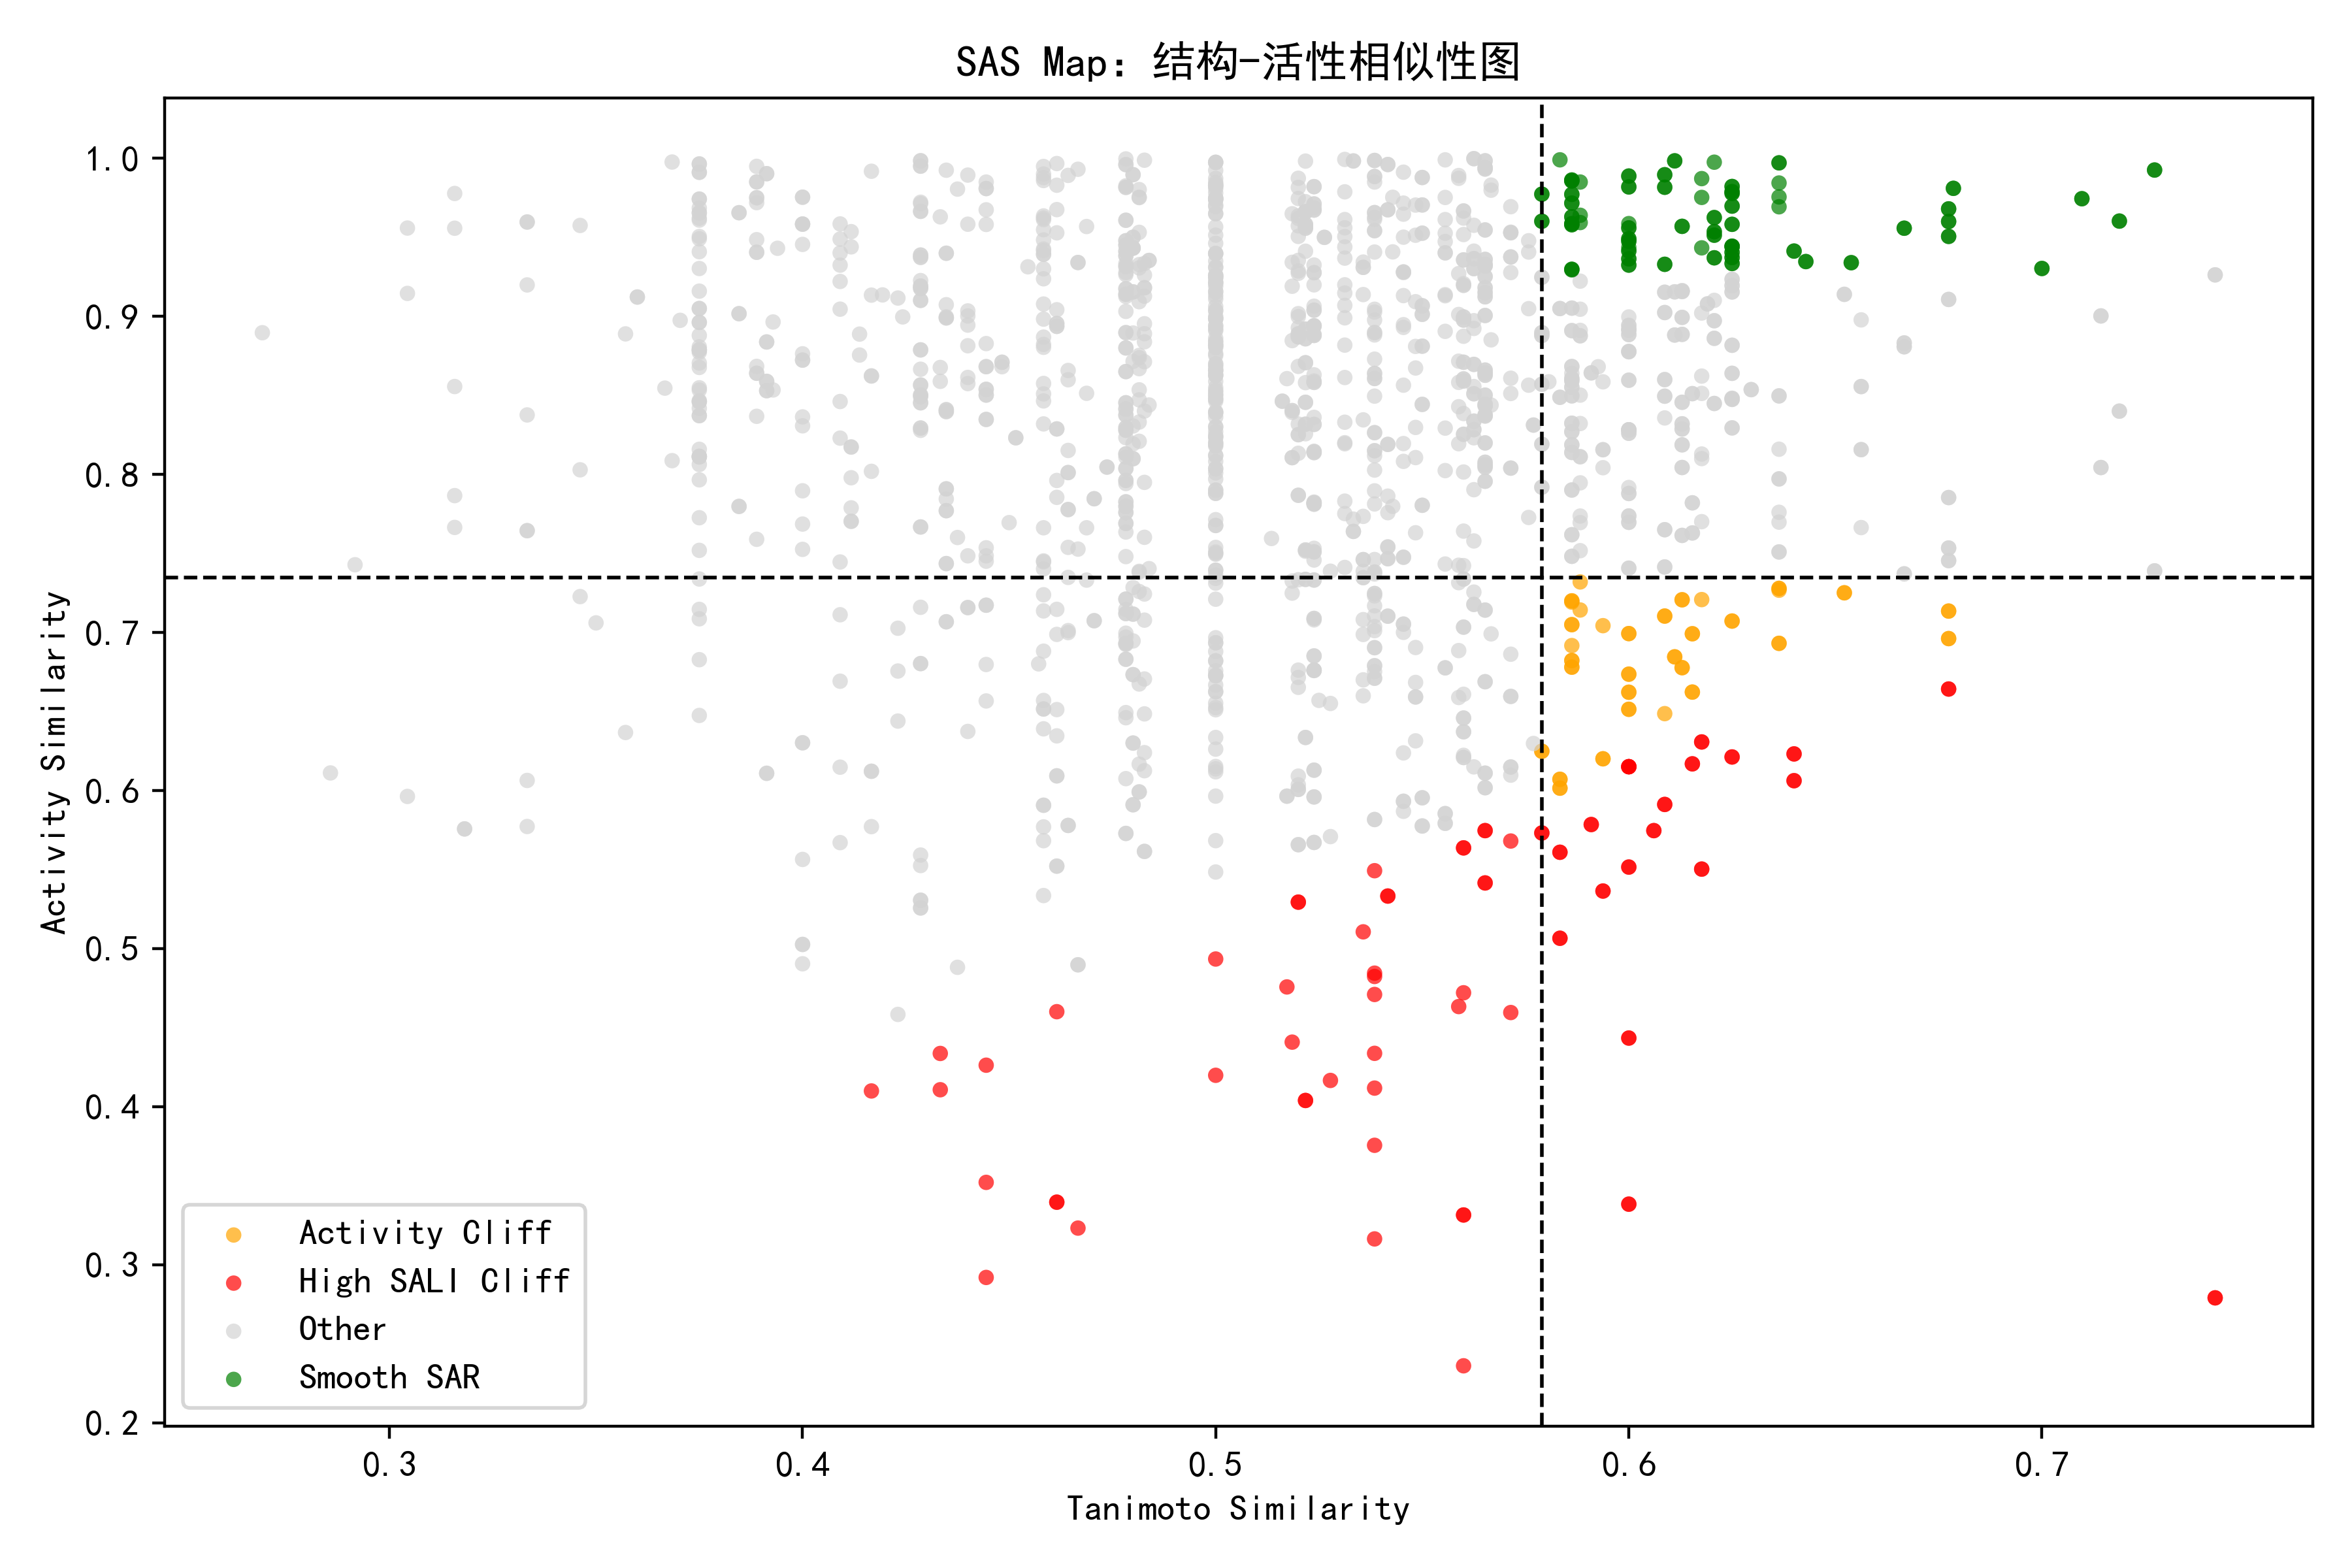
\includegraphics[width=0.82\textwidth]{问题2_SAS结构活性相似性图.png}
\caption{基于 KNN 图的结构—活性相似性图}
\end{figure}

图 4 中右下方区域对应结构相似度较高但活性相似度较低的分子对，即典型活性悬崖区域。图中既存在结构相似且活性相似的平滑结构—活性关系分子对，也存在结构相似但活性显著不同的活性悬崖分子对。

\begin{figure}[H]
\centering
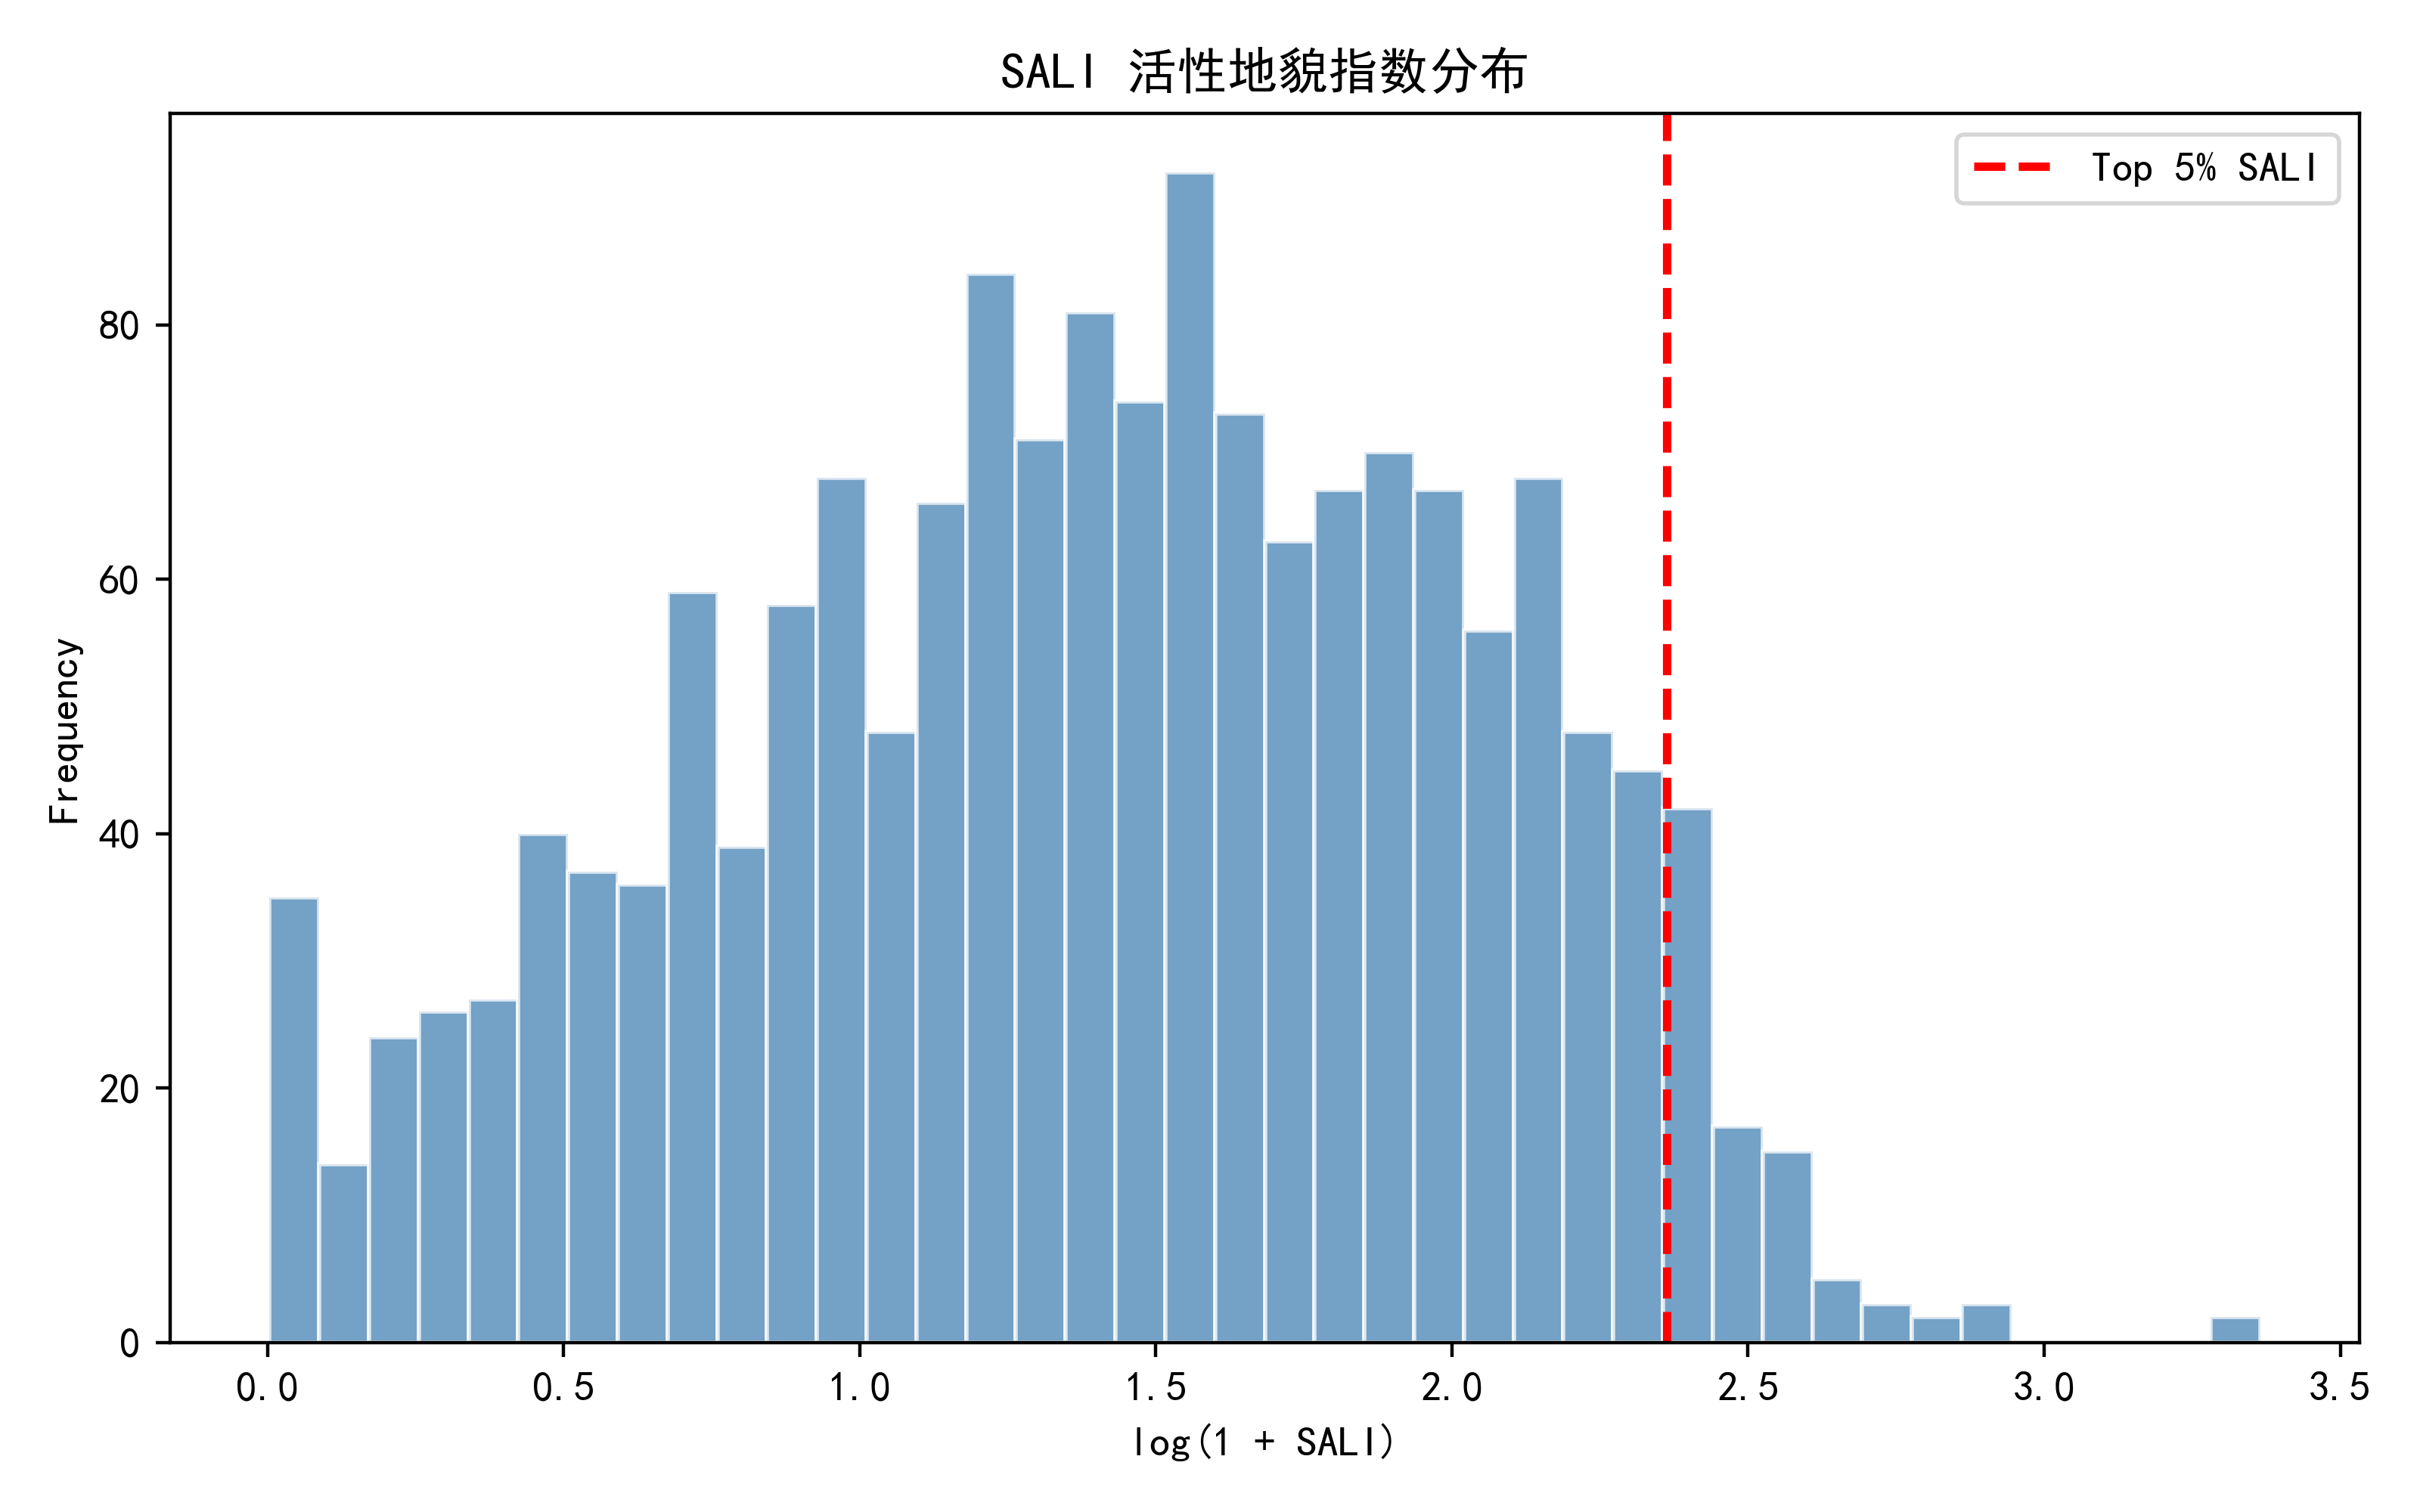
\includegraphics[width=0.82\textwidth]{问题2_SALI活性悬崖指数分布图.png}
\caption{SALI 活性悬崖指数分布}
\end{figure}

由于 SALI 取值跨度较大，图 5 采用 $\log(1+SALI)$ 进行可视化。结果显示绝大多数分子对集中在中低 SALI 区域，而右侧存在少量高 SALI 分子对，说明整体结构—活性关系以平缓变化为主，但局部区域仍存在显著活性悬崖。

部分高 SALI 活性悬崖分子对如下。

\begin{table}[H]
\centering
\caption{部分高 SALI 活性悬崖分子对}
\small
\resizebox{\textwidth}{!}{%
\begin{tabular}{llllllllll}
\toprule
Source & Target & Mol1\_ID & Mol2\_ID & Mol1\_Activity & Mol2\_Activity & Tanimoto 相似度 & 活性差异 & SALI & 类型 \\
\midrule
319 & 94 & 319 & 94 & 8.4640 & 1.2551 & 0.7419 & 7.2090 & 27.9347 & High SALI Cliff \\
94 & 319 & 94 & 319 & 1.2551 & 8.4640 & 0.7419 & 7.2090 & 27.9347 & High SALI Cliff \\
109 & 297 & 109 & 297 & 8.5581 & 0.9192 & 0.5600 & 7.6389 & 17.3611 & High SALI Cliff \\
304 & 109 & 304 & 109 & 1.9419 & 8.5581 & 0.6000 & 6.6162 & 16.5405 & High SALI Cliff \\
109 & 304 & 109 & 304 & 8.5581 & 1.9419 & 0.6000 & 6.6162 & 16.5405 & High SALI Cliff \\
38 & 297 & 38 & 297 & 7.6039 & 0.9192 & 0.5600 & 6.6847 & 15.1925 & High SALI Cliff \\
297 & 38 & 297 & 38 & 0.9192 & 7.6039 & 0.5600 & 6.6847 & 15.1925 & High SALI Cliff \\
111 & 109 & 111 & 109 & 1.7220 & 8.5581 & 0.5385 & 6.8361 & 14.8116 & High SALI Cliff \\
54 & 110 & 54 & 110 & 1.3527 & 6.9181 & 0.6000 & 5.5653 & 13.9134 & High SALI Cliff \\
110 & 54 & 110 & 54 & 6.9181 & 1.3527 & 0.6000 & 5.5653 & 13.9134 & High SALI Cliff \\
\bottomrule
\end{tabular}%
}
\end{table}

其中，分子 319 与分子 94 的 Tanimoto 相似度为 0.7419，但活性得分分别为 8.4640 和 1.2551，活性差异达到 7.2090，SALI 值为 27.9347，是典型的强活性悬崖分子对。

\subsection{分子局部敏感度模型}

分子对层面的 SALI 指数只能描述两个分子之间的局部突变强度。已有研究进一步将活性悬崖组织为网络或相似图，用节点及其邻接关系刻画局部 SAR 不连续性\cite{ref:guha2012landscape}。为了刻画单个分子在其相似邻域内的整体活性波动程度，定义分子 $i$ 的相似邻域为

\[
N(i)=\{j:(i,j)\in E\},
\]

其中 $E$ 为 KNN 相似图边集合。基于此，定义分子 $i$ 的局部敏感度为

\[
LS_i=\frac{1}{|N(i)|}\sum_{j\in N(i)}SALI_{ij}.
\]

该指标表示分子 $i$ 与其相似邻居之间的平均活性悬崖强度。若 $LS_i$ 较大，说明该分子附近的结构—活性关系较陡峭，小范围结构变化可能引起较大活性波动；若 $LS_i$ 较小，则说明其局部邻域内结构—活性关系较平滑，稳定性较好。

此外，本文统计每个分子参与活性悬崖的次数 \texttt{Cliff\_Count}，作为局部敏感性的辅助评价指标。

\begin{table}[H]
\centering
\caption{局部敏感度较高的代表分子}
\small
\resizebox{\textwidth}{!}{%
\begin{tabular}{llllllll}
\toprule
Index & ID & Bioactivity\_Score & Local\_Sensitivity & Max\_Local\_SALI & Neighbor\_Count & Cliff\_Count & Region \\
\midrule
94 & 94 & 1.2551 & 14.7412 & 27.9347 & 7 & 5 & Ordinary \\
319 & 319 & 8.4640 & 11.7217 & 27.9347 & 10 & 7 & Hotspot \\
51 & 51 & 10.0000 & 11.5475 & 12.7438 & 6 & 6 & Ordinary \\
109 & 109 & 8.5581 & 11.2144 & 17.3611 & 14 & 11 & Ordinary \\
196 & 196 & 8.4946 & 9.9044 & 11.7596 & 7 & 5 & Hotspot \\
54 & 54 & 1.3527 & 9.6046 & 13.9134 & 13 & 8 & Ordinary \\
95 & 95 & 1.2173 & 9.0166 & 12.6089 & 6 & 2 & Ordinary \\
38 & 38 & 7.6039 & 8.8630 & 15.1925 & 9 & 5 & Ordinary \\
282 & 282 & 1.9043 & 8.1346 & 11.9974 & 9 & 5 & Ordinary \\
55 & 55 & 7.3069 & 7.8619 & 11.1684 & 10 & 3 & Hotspot \\
\bottomrule
\end{tabular}%
}
\end{table}

局部敏感度较高的分子既包含低活性分子，也包含高活性分子。例如，分子 94 的活性得分仅为 1.2551，但局部敏感度达到 14.7412；分子 319 的活性得分为 8.4640，局部敏感度也达到 11.7217。这说明局部敏感性并不完全由分子自身活性决定，而更多反映其相似邻域内结构—活性地貌的陡峭程度。

\subsection{不同空间分区的稳定性比较}

结合第一问得到的 Hotspot 与 Ordinary 标签，统计不同区域的平均活性、局部敏感度和参与悬崖次数，结果如下。

\begin{table}[H]
\centering
\caption{不同空间分区的活性与局部敏感度统计}
\small
\resizebox{\textwidth}{!}{%
\begin{tabular}{llllll}
\toprule
区域 & 分子数 & 平均活性 & 平均局部敏感度 & 中位局部敏感度 & 平均参与悬崖次数 \\
\midrule
Hotspot & 82 & 6.2061 & 3.9907 & 3.5296 & 0.9878 \\
Ordinary & 243 & 4.1201 & 3.8726 & 3.5109 & 0.8107 \\
\bottomrule
\end{tabular}%
}
\end{table}

热点区域的平均活性显著高于普通区域，与第一问结论一致。从局部敏感度看，热点区域平均局部敏感度为 3.9907，普通区域为 3.8726，热点区域略高于普通区域；但两者中位局部敏感度分别为 3.5296 和 3.5109，差异较小。这说明热点区域虽具有更高活性，但整体稳定性并未显著低于普通区域。

\begin{figure}[H]
\centering
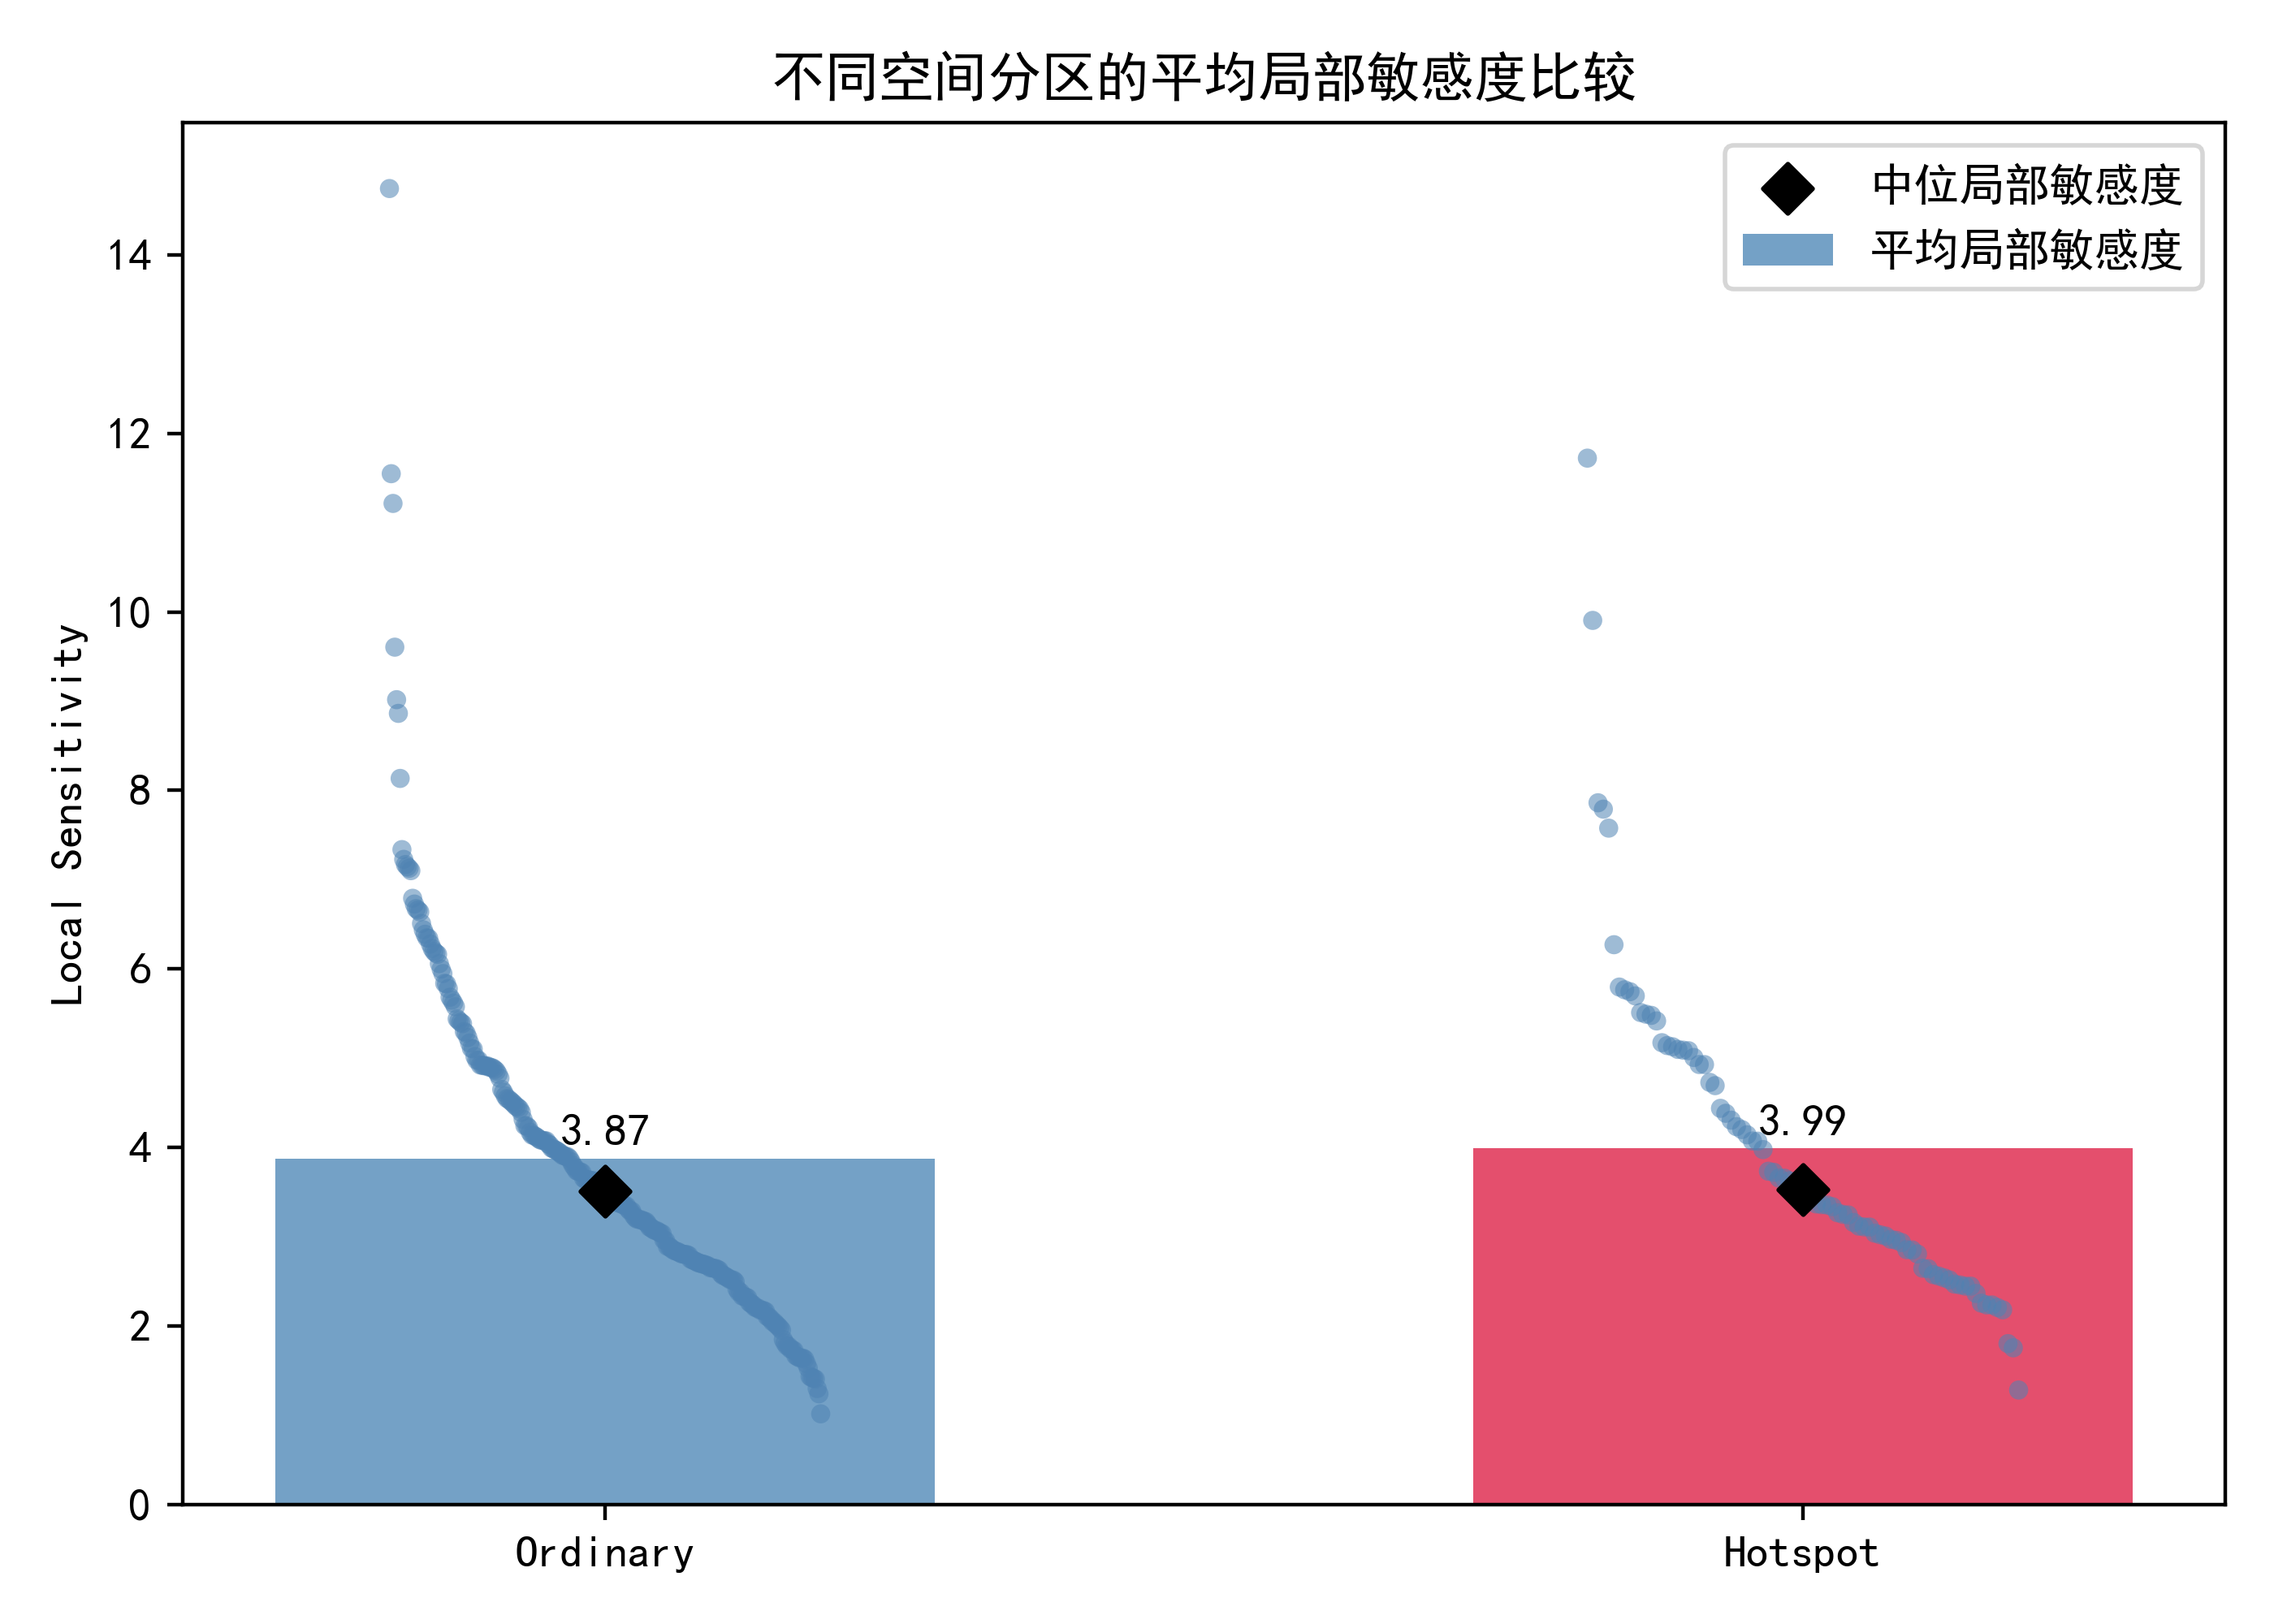
\includegraphics[width=0.82\textwidth]{问题2_不同区域平均局部敏感度柱状图.png}
\caption{不同空间分区的平均局部敏感度比较}
\end{figure}

图 6 显示，热点区域的平均局部敏感度略高于普通区域，但差异并不明显；普通区域中也存在若干局部敏感度较高的分子。因此，后续候选分子筛选不应仅依据空间区域或活性水平，还应结合单个分子的局部敏感度进行综合判断。

\subsection{高活性与局部敏感度关联分析}

为了分析高活性与高局部敏感度之间是否存在明显关联，计算分子活性得分 $A_i$ 与局部敏感度 $LS_i$ 的 Pearson 相关系数：

\[
r=corr(A_i,LS_i).
\]

计算得到

\[
r=0.112.
\]

该值接近 0，说明分子活性得分与局部敏感度之间仅存在很弱的正相关关系，并不存在明显线性关联。

\begin{figure}[H]
\centering
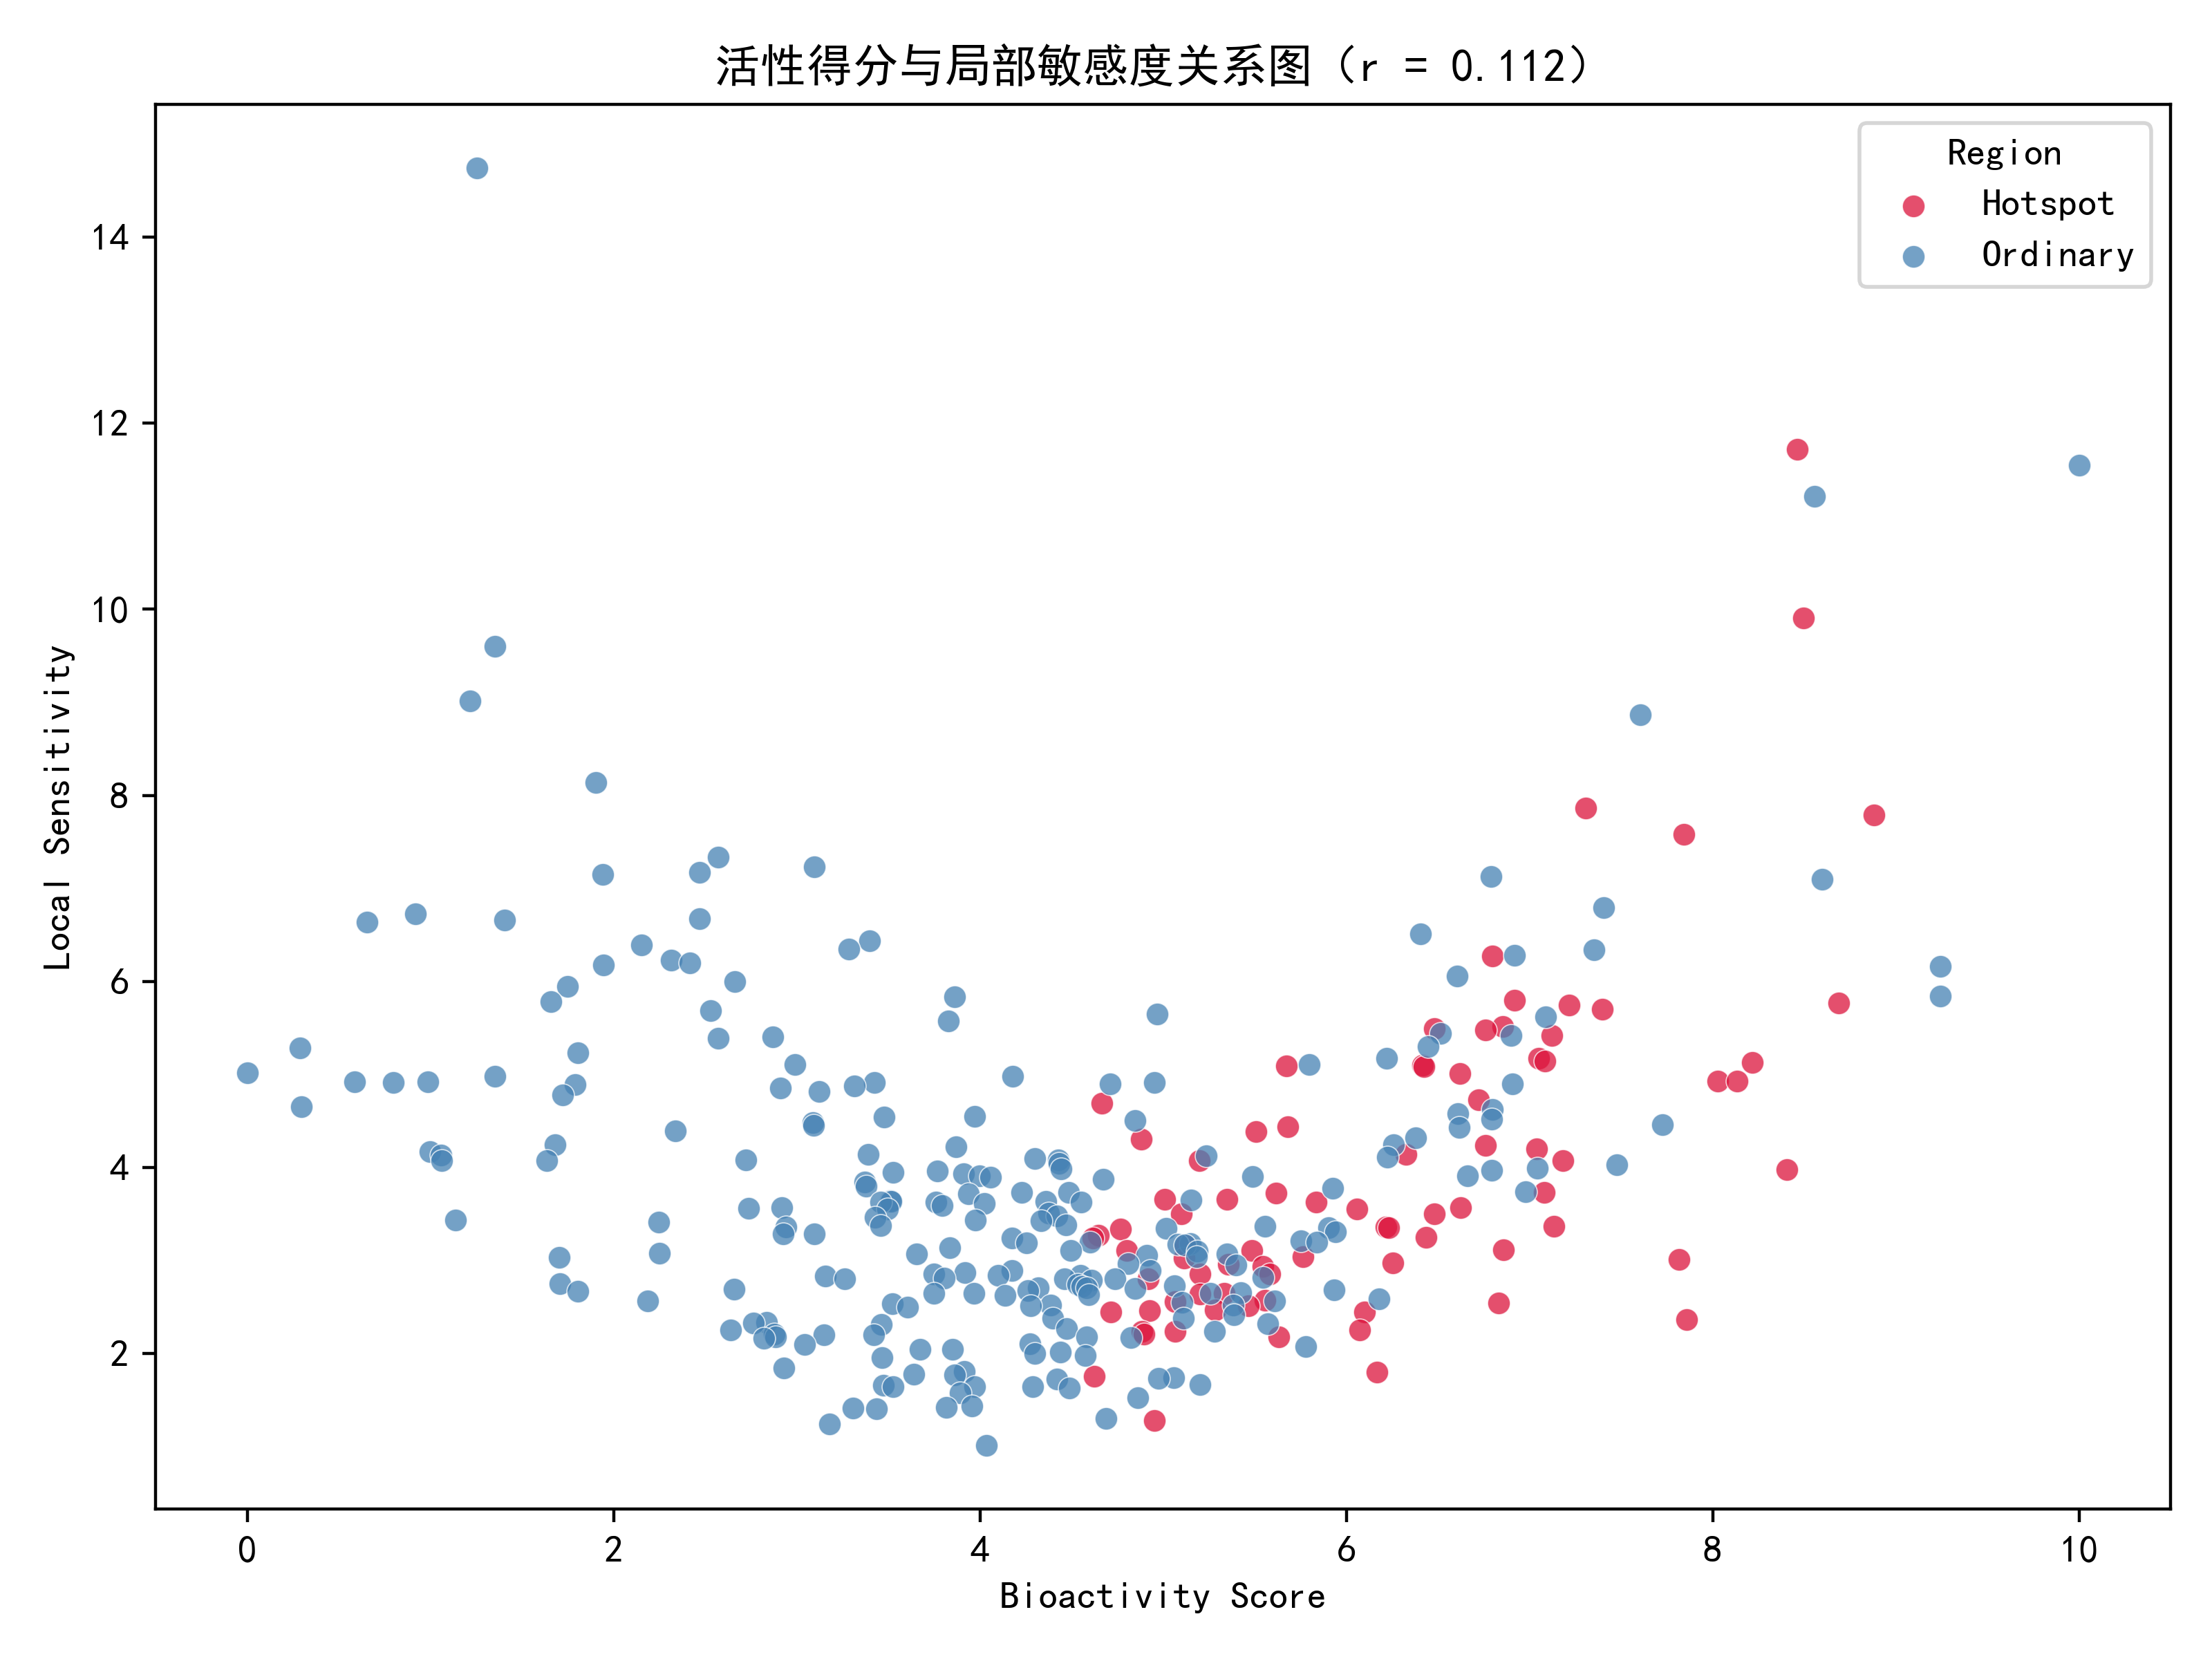
\includegraphics[width=0.82\textwidth]{问题2_活性得分与局部敏感度关系图.png}
\caption{活性得分与局部敏感度关系}
\end{figure}

图 7 中热点区域分子主要分布在较高活性区间，但其局部敏感度差异较大；普通区域中也存在若干局部敏感度较高的分子。整体点云没有明显单调上升趋势，与相关系数 $r=0.112$ 的结果一致。因此，高活性分子并不必然对应高局部敏感度，这为第三问中筛选高活性且低敏感的稳健分子提供了可能。


\section{问题三：下一轮实验候选分子优选}

\subsection{多目标优选模型}

下一轮实验预算仅允许验证 8 个分子。若只按照生物活性排序，可能选入局部敏感度较高、研发风险较大的分子；若过分强调稳定性或多样性，则可能牺牲过多活性。多目标参考化合物选择研究指出，固定规模候选集合的构造本质上涉及结构、理化性质和响应覆盖之间的显式权衡\cite{ref:ohto2026multiobjective}。因此，本文将候选分子筛选建模为固定集合大小的多目标组合优化问题。

记全部候选分子集合为

\[
D=\{1,2,\cdots,N\},
\]

需要从中选出 8 个分子构成实验验证集合：

\[
S\subset D,\quad |S|=8.
\]

\subsubsection{平均活性目标}

定义候选集合 $S$ 的平均活性为

\[
F_1(S)=\frac{1}{8}\sum_{i\in S}A_i.
\]

该指标越大，说明所选分子的整体生物活性越高。由于候选分子最终仍需进入实验验证，高活性仍是优先筛选的基础目标；但活性地貌研究提示高活性点附近可能同时存在局部不连续风险\cite{ref:guha2012landscape}。因此该目标的优化方向为

\[
F_1(S)\rightarrow \max.
\]

\subsubsection{局部敏感性目标}

定义候选集合 $S$ 的平均局部敏感度为

\[
F_2(S)=\frac{1}{8}\sum_{i\in S}LS_i.
\]

该指标越小，说明集合整体结构—活性关系越稳定，优化方向为

\[
F_2(S)\rightarrow \min.
\]

\subsubsection{结构近邻冗余目标}

为避免入选分子在结构上过于重复，参考多目标化合物选择中通过降低集合内结构相似度提升结构覆盖的思想\cite{ref:ohto2026multiobjective}，定义集合 $S$ 内部平均近邻结构相似度为

\[
F_3(S)=\frac{2}{8(8-1)}\sum_{i<j,\ i,j\in S}sim(i,j).
\]

若分子对 $(i,j)$ 在 KNN 图中存在边，则使用其对应的 Tanimoto 相似度；若二者并非近邻，则在近邻冗余评价中记为 0。需要指出的是，此处的 0 并不表示真实 Tanimoto 相似度为 0，而表示二者在给定 KNN 相似图中不存在局部近邻冗余关系。该指标越小，说明所选分子之间近邻冗余越低，结构多样性越好，优化方向为

\[
F_3(S)\rightarrow \min.
\]

\subsubsection{空间分散度目标}

题目要求入选分子之间具有一定多样性，避免过于集中在同一局部区域。本文采用集合内分子两两欧氏距离的平均值刻画二维流形空间分散程度。定义

\[
d_{ij}=\|X_i-X_j\|_2=\sqrt{(x_i-x_j)^2+(y_i-y_j)^2},
\]

则集合 $S$ 的空间分散度为

\[
F_4(S)=\frac{2}{8(8-1)}\sum_{i<j,\ i,j\in S}d_{ij}.
\]

该指标越大，说明所选分子在二维流形空间中覆盖范围越广，优化方向为

\[
F_4(S)\rightarrow \max.
\]

\subsubsection{理化性质多样性辅助评价}

设分子 $i$ 的理化性质向量为

\[
p_i=(LogP_i,TPSA_i,MolWt_i,Dipole_i,Charge_i,BalabanJ_i,BertzCT_i).
\]

LogP、TPSA、分子量等理化性质常用于刻画化合物空间覆盖和潜在药物性质，其中 TPSA 等描述符也被广泛用于分子转运性质和化合物筛选分析\cite{ref:ohto2026multiobjective}。对各维指标标准化后，定义集合 $S$ 的理化性质分散度为

\[
F_5(S)=\frac{2}{8(8-1)}\sum_{i<j,\ i,j\in S}\|p_i-p_j\|_2.
\]

该指标不直接参与核心优化，而用于检验最终推荐集合是否具有较好的理化性质覆盖能力。

\subsection{多目标遗传算法求解}

多目标遗传算法特别是 NSGA-II 常用于在多个相互冲突目标之间搜索非支配解集\cite{ref:deb2002nsga2}。为统一优化方向，将目标函数转换为全部最大化形式：

\[
G_1(S)=F_1(S),
\]

\[
G_2(S)=-F_2(S),
\]

\[
G_3(S)=-F_3(S),
\]

\[
G_4(S)=F_4(S).
\]

因此，多目标优化形式为

\[
(G_1(S),G_2(S),G_3(S),G_4(S))\rightarrow \max.
\]

遗传算法中的每个个体表示一个包含 8 个不同分子的候选集合：

\[
S=\{i_1,i_2,\cdots,i_8\}.
\]

算法基本步骤如下：

\begin{enumerate}
\item 随机生成初始种群，同时引入由高活性、低敏感性分子构成的初始个体，提高搜索效率；
\item 对每个个体计算 $F_1$、$F_2$、$F_3$ 和 $F_4$；
\item 根据非支配排序确定 Pareto 等级，并结合拥挤距离保持解集多样性，这是 NSGA-II 保持前沿分布均匀性的核心机制\cite{ref:deb2002nsga2}；
\item 通过交叉操作交换父代集合中的部分分子，生成新候选组合；
\item 通过变异操作随机替换集合中的一个或两个分子，扩大搜索空间；
\item 对交叉和变异后出现重复编号的个体进行修正，保证 $|S|=8$ 且分子编号不重复；
\item 迭代结束后，从所有候选方案中提取 Pareto 前沿解。

\end{enumerate}
本文共生成 11870 个不同候选方案，其中 Pareto 前沿方案 2785 个。较多的非支配方案说明活性、局部敏感性和多样性目标之间存在明显权衡关系，需要进一步从 Pareto 前沿中选择唯一推荐方案。

\subsection{Pareto 前沿方案选择}

对 Pareto 前沿方案中的 $F_1$、$F_2$、$F_3$ 和 $F_4$ 分别进行 0—1 归一化，记为 $\widetilde{F_1}$、$\widetilde{F_2}$、$\widetilde{F_3}$ 和 $\widetilde{F_4}$。综合评分定义为

\[
Score(S)=0.40\widetilde{F_1}(S)-0.30\widetilde{F_2}(S)-0.15\widetilde{F_3}(S)+0.15\widetilde{F_4}(S).
\]

其中，活性权重设置为 0.40，体现活性作为实验优先级核心指标的重要性；局部敏感度权重设置为 0.30，用于控制活性悬崖风险；结构近邻冗余和空间分散度权重均为 0.15，用于保证结构和空间多样性。类似地，Ohto 等在多目标参考化合物选择中也将综合评分作为从 Pareto 前沿中选取展示性方案的后处理步骤，而非替代非支配解集本身\cite{ref:ohto2026multiobjective}。该综合评分仅用于从 Pareto 前沿中选取最终方案，并不替代前述多目标优化过程。

最终选择 Pareto 前沿中综合评分最高的方案：

\[
S^*=\arg\max_{S\in Pareto}Score(S).
\]

\subsection{优化结果分析}

遗传算法搜索过程中的种群平均指标变化如下图所示。

\begin{figure}[H]
\centering
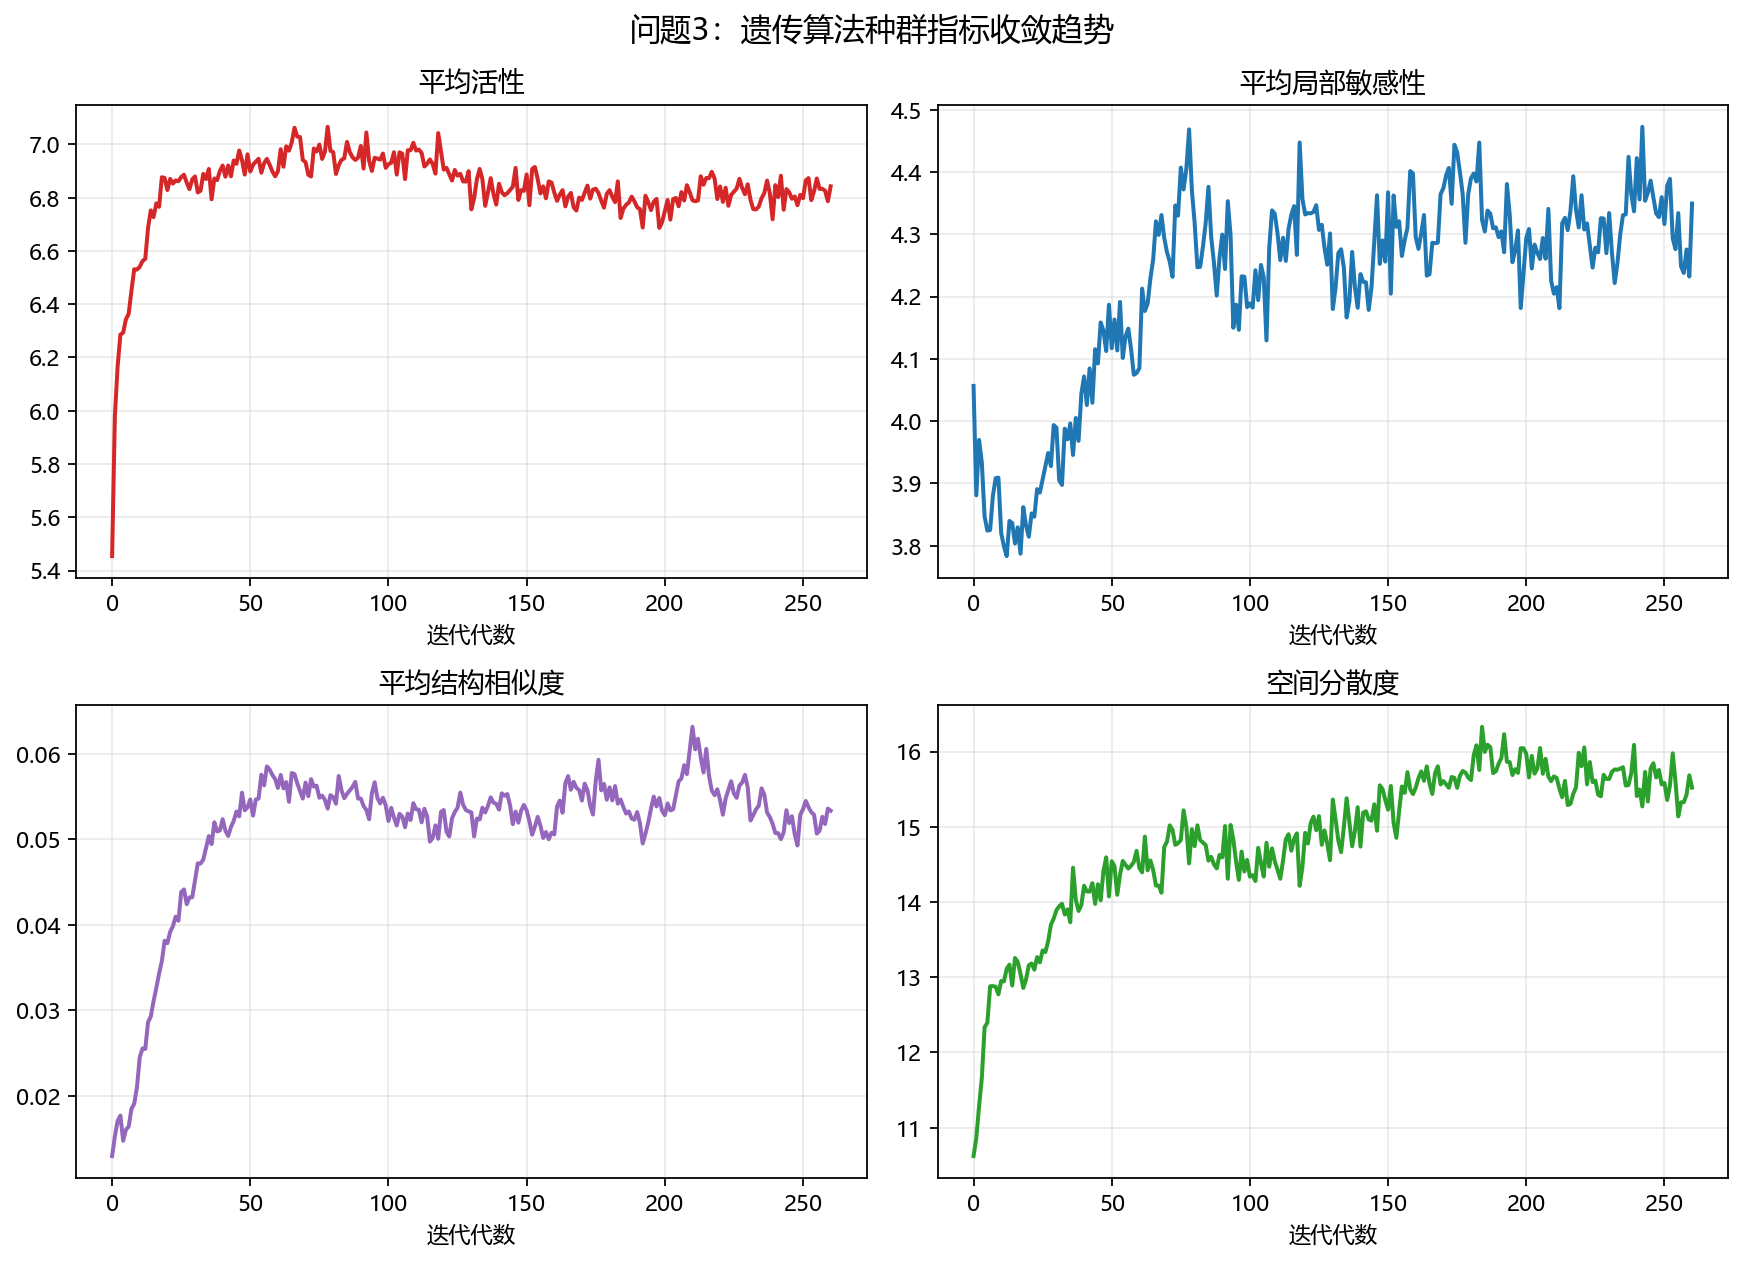
\includegraphics[width=0.82\textwidth]{问题3_遗传算法收敛趋势.png}
\caption{多目标遗传算法迭代过程中的种群平均指标变化}
\end{figure}

图 8 显示，平均活性在迭代前期迅速上升，并在后期保持在较高水平，说明遗传算法能够有效筛选出活性较优的候选组合。空间分散度也随迭代明显提高，表明算法逐渐倾向于选择覆盖范围更广的分子集合。平均局部敏感度和平均结构相似度在迭代过程中存在一定波动，反映出高活性、低风险和多样性目标之间存在权衡关系。

\begin{figure}[H]
\centering
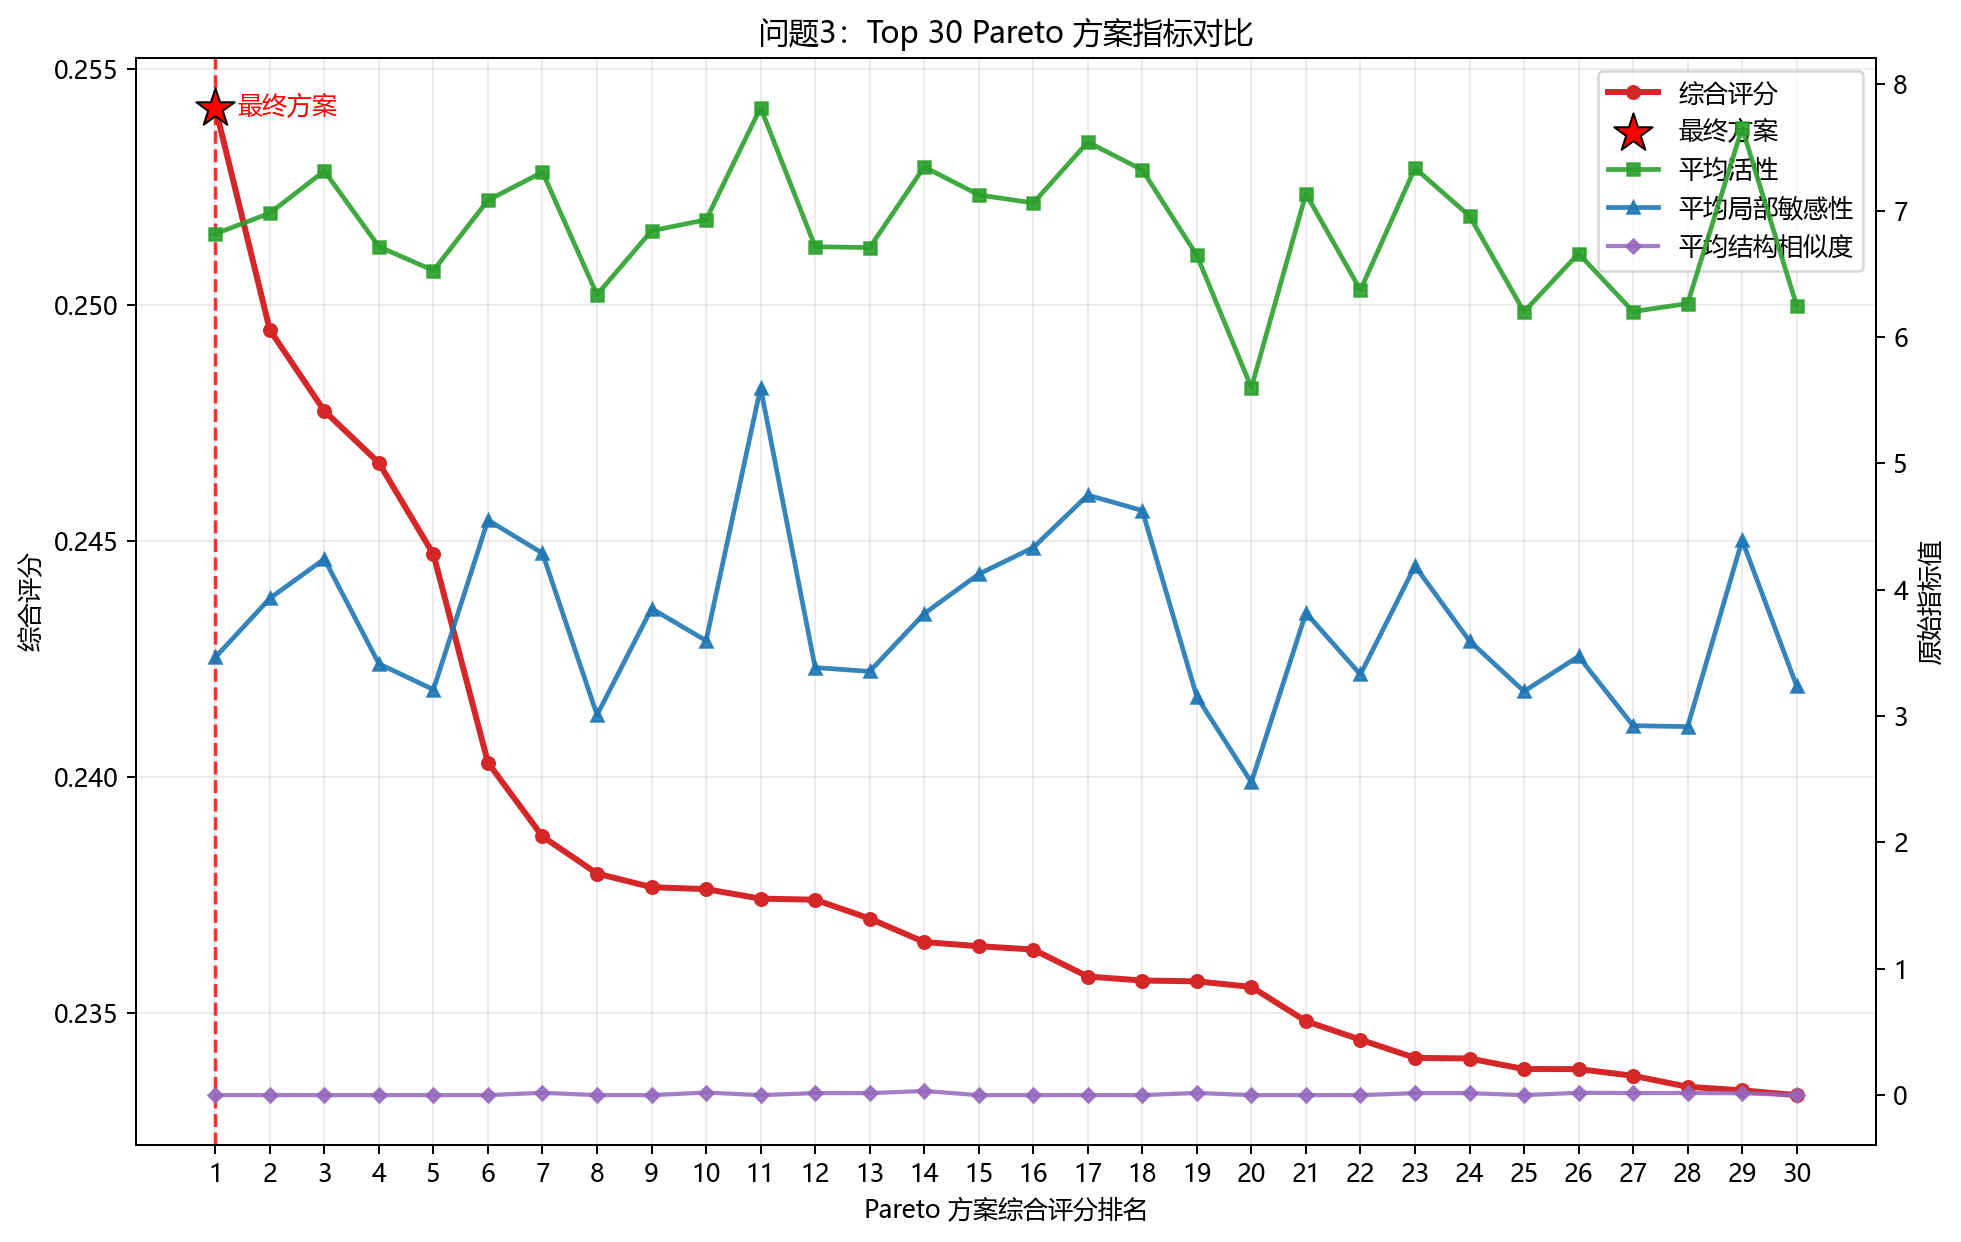
\includegraphics[width=0.82\textwidth]{问题3_Pareto前沿分布.png}
\caption{Pareto 前沿 Top 30 方案的综合指标比较}
\end{figure}

图 9 表明，排名靠前的 Pareto 方案整体具有较高综合评分，但活性、敏感性和结构相似度并非完全同步变化。最终方案位于综合评分最高位置，因此被选为下一轮实验优先验证的 8 分子组合。

最终推荐候选分子集合为

\[
S^*=\{1,12,86,101,118,140,236,318\}.
\]

其集合层面的主要指标如下。

\begin{table}[H]
\centering
\caption{最终推荐方案的集合层面指标}
\small
\resizebox{\textwidth}{!}{%
\begin{tabular}{lll}
\toprule
指标 & 数值 & 说明 \\
\midrule
平均活性 & 6.8153 & 高于全体分子平均活性 4.6465 \\
平均局部敏感度 & 3.4643 & 低于全体平均局部敏感度 3.9024 \\
平均结构相似度 & 0.0000 & 在 KNN 图中内部近邻冗余较低 \\
二维空间分散度 & 16.9614 & 高于全体平均空间分散度 12.2460 \\
理化性质分散度 & 3.9157 & 高于全体平均理化性质分散度 3.5015 \\
综合评分 & 0.2542 & Pareto 前沿中综合评分最高 \\
\bottomrule
\end{tabular}%
}
\end{table}

推荐集合的平均活性达到 6.8153，明显高于全体分子平均活性 4.6465，也高于第一问中普通区域平均活性 4.1201。同时，该集合平均局部敏感度为 3.4643，低于全体平均值 3.9024，说明其在保持较高活性的同时整体风险较低。集合内部平均结构相似度为 0，表示这些分子在 KNN 图中不存在明显近邻冗余；二维空间分散度为 16.9614，高于全体平均水平，说明所选分子在流形空间中覆盖范围较广。

\subsection{与基准方案比较}

为说明推荐方案相对于简单活性排序的优势，本文将其与“仅按活性前 8”的方案进行比较。

\begin{table}[H]
\centering
\caption{推荐方案与基准方案指标比较}
\small
\resizebox{\textwidth}{!}{%
\begin{tabular}{llllll}
\toprule
方案 & 平均活性 & 平均局部敏感度 & 平均结构相似度 & 空间分散度 & 理化性质分散度 \\
\midrule
全体平均 & 4.6465 & 3.9024 & 0.0110 & 12.2460 & 3.5015 \\
仅按活性前 8 & 8.9634 & 8.1662 & 0.0000 & 8.3726 & 3.3529 \\
本文推荐 8 个 & 6.8153 & 3.4643 & 0.0000 & 16.9614 & 3.9157 \\
\bottomrule
\end{tabular}%
}
\end{table}

仅按活性排序得到的前 8 个分子虽然平均活性最高，但其平均局部敏感度达到 8.1662，明显高于本文推荐方案，说明其中可能包含较多活性悬崖附近的高风险分子。同时，该方案空间分散度仅为 8.3726，说明分布较为集中。相比之下，本文推荐方案适当牺牲部分平均活性，显著降低了局部敏感性，并提高了空间分散度和理化性质分散度，更符合题目要求的“高活性、低敏感性和一定多样性”的综合原则。

\begin{figure}[H]
\centering
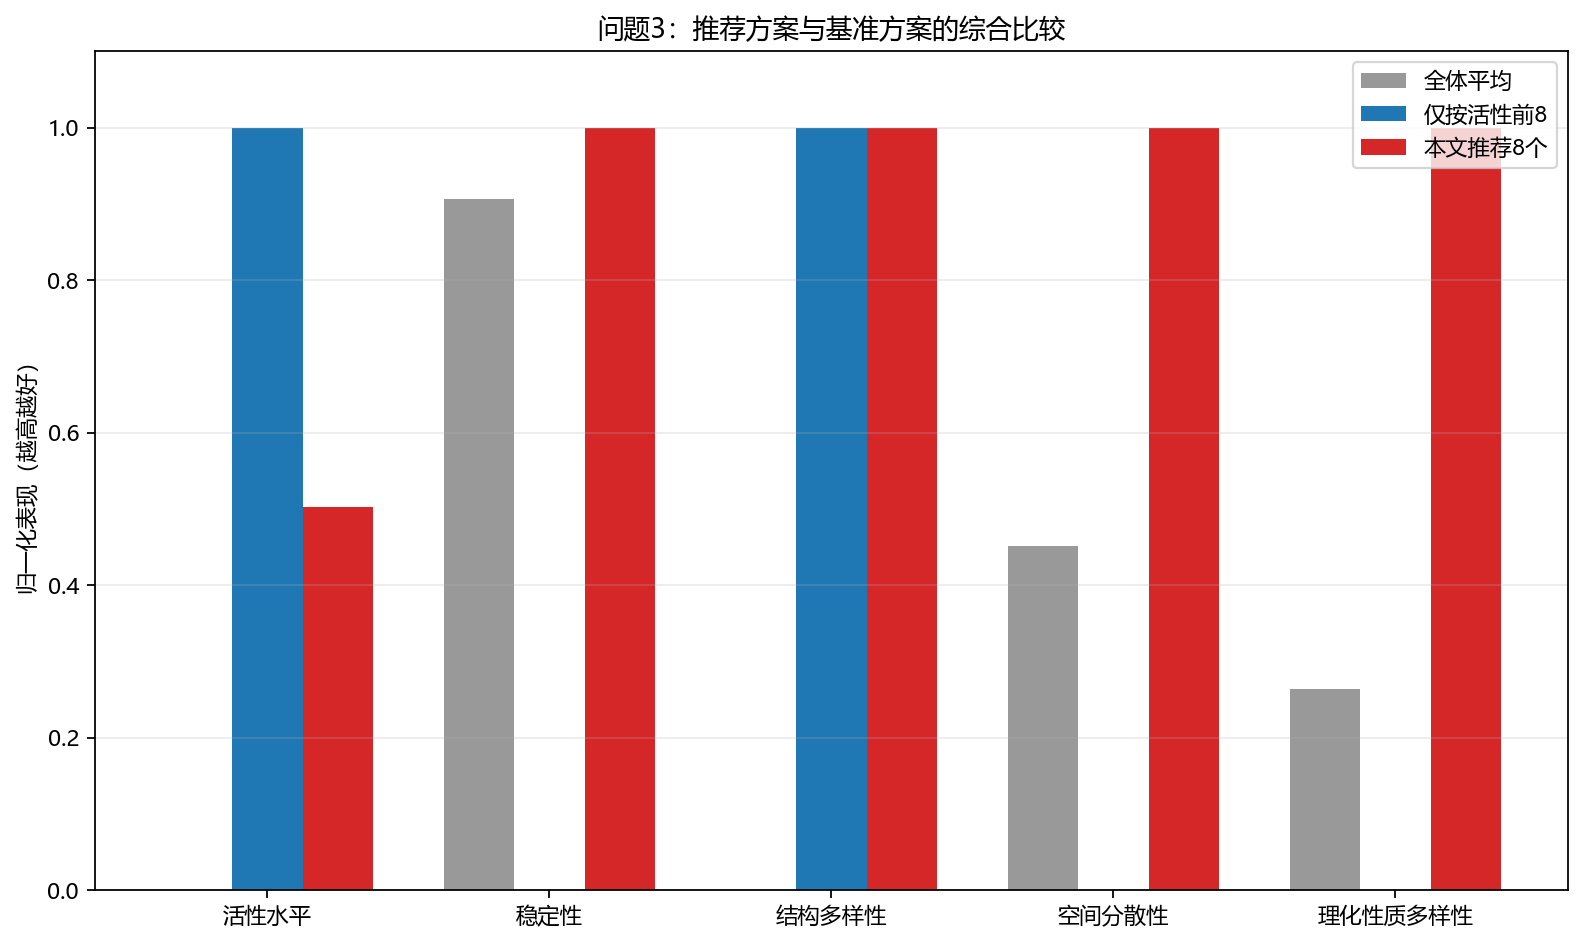
\includegraphics[width=0.82\textwidth]{问题3_推荐方案指标对比.png}
\caption{推荐方案与基准方案的归一化指标比较}
\end{figure}

\subsection{推荐分子解释}

最终推荐的 8 个分子具体信息如下。

\begin{table}[H]
\centering
\caption{最终推荐 8 个分子的具体信息}
\small
\resizebox{\textwidth}{!}{%
\begin{tabular}{llllllll}
\toprule
分子 ID & SMILES & 区域 & 热点编号 & 活性得分 & 局部敏感度 & 悬崖次数 & 选择说明 \\
\midrule
1 & COc1ccc2ccccc2c1 & Ordinary & -1 & 9.2424 & 6.1639 & 0 & 活性很高，虽敏感度偏高但未参与活性悬崖 \\
12 & COc1ncc2ncn(C)c2n1 & Hotspot & 4 & 6.1003 & 2.4481 & 0 & 热点区域分子，活性与稳定性较均衡 \\
86 & C=Cc1cccc(C(C)C)c1 & Hotspot & 10 & 6.1681 & 1.8044 & 0 & 局部敏感度较低，可提高稳定性 \\
101 & Nc1ccc2ccccc2c1 & Hotspot & 0 & 8.4053 & 3.9776 & 0 & 高活性热点区域代表分子 \\
118 & CC(CS(N)(=O)=O)c1ccccc1 & Hotspot & 3 & 6.8332 & 2.5413 & 0 & 活性较高且敏感性较低 \\
140 & CCC(C)N1CCNCC1 & Ordinary & -1 & 3.8930 & 1.5797 & 0 & 活性一般但稳定性好，并显著增加空间多样性 \\
236 & OCCn1cnc2cncnc21 & Hotspot & 8 & 6.4808 & 3.5006 & 0 & 热点区域分子，综合表现稳定 \\
318 & C\#CC1CCCCC1 & Hotspot & 11 & 7.3994 & 5.6987 & 0 & 活性较高，补充另一空间区域 \\
\bottomrule
\end{tabular}%
}
\end{table}

从区域分布看，8 个分子中有 6 个来自第一问识别出的热点区域，说明推荐方案主要保留了高活性热点中的优质分子；同时有 2 个来自普通区域，其中分子 1 具有很高活性，分子 140 虽活性相对一般，但局部敏感度较低且在二维空间中位置较为独立，对提高整体空间覆盖具有贡献。该结果体现出模型并非机械选择热点分子或高活性分子，而是在活性、稳定性和多样性之间进行综合权衡。

\begin{figure}[H]
\centering
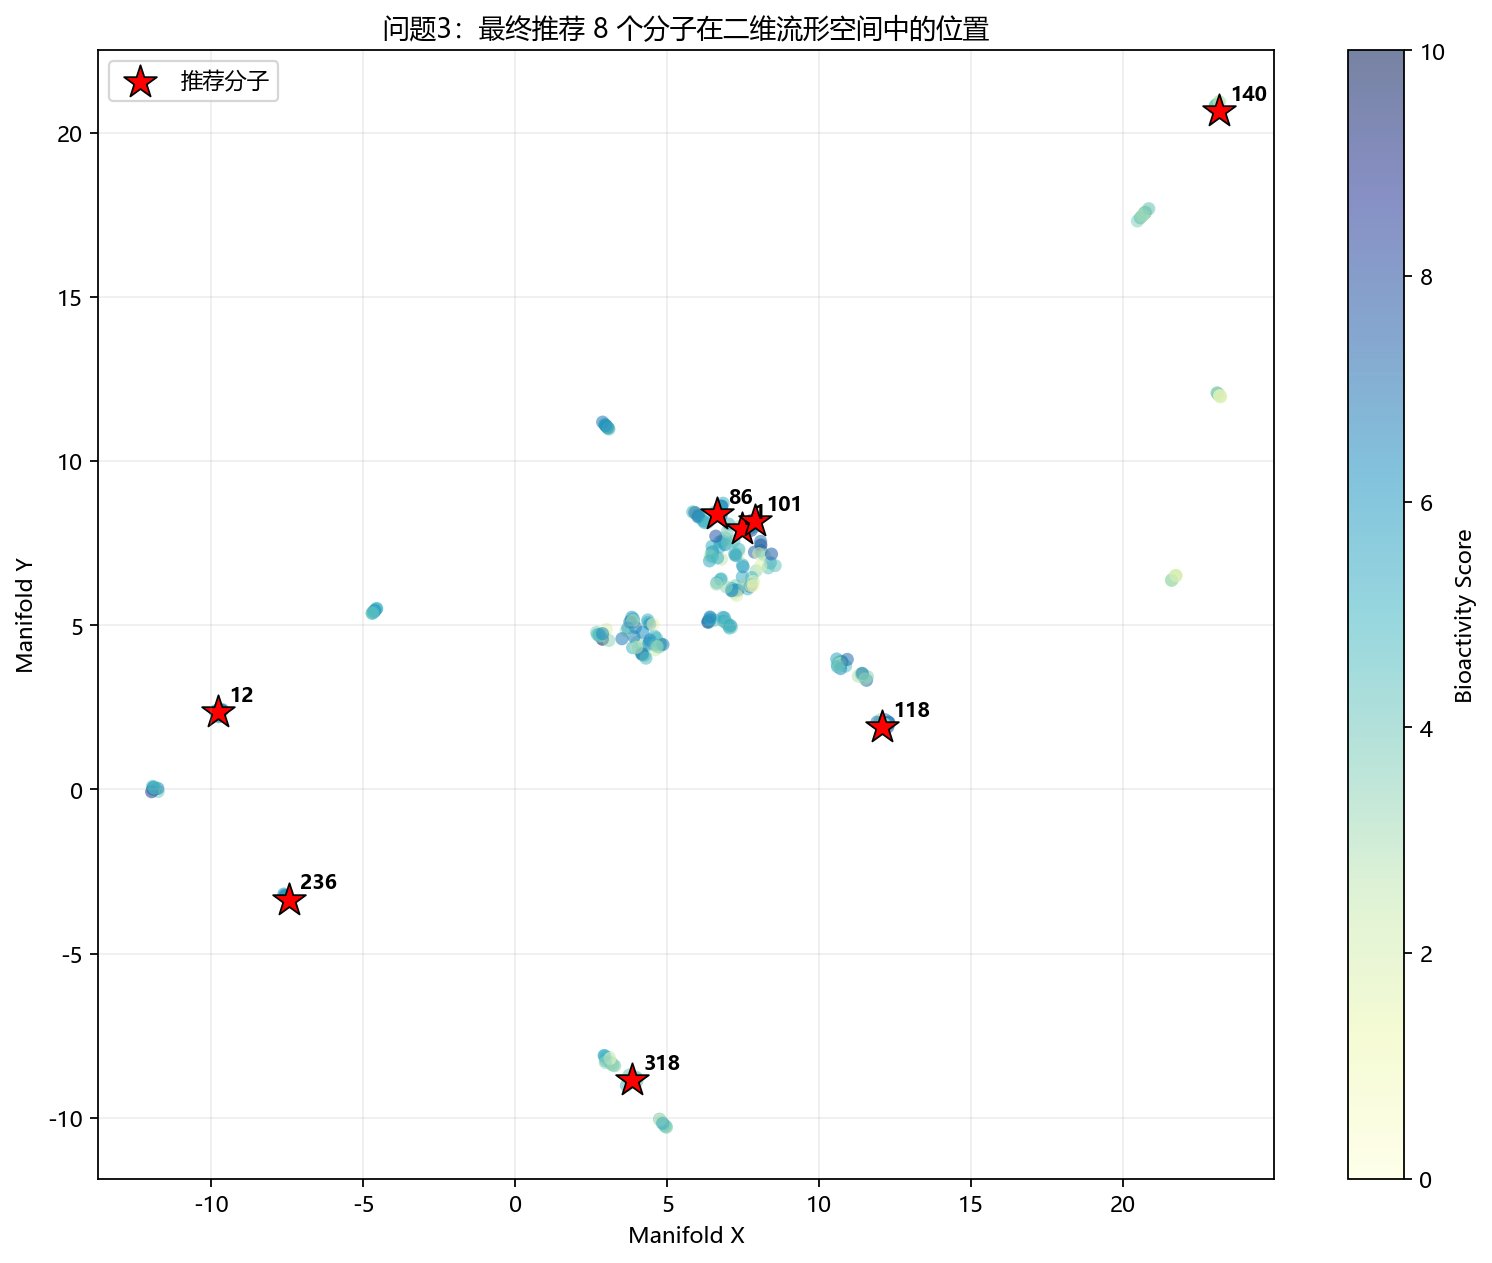
\includegraphics[width=0.82\textwidth]{问题3_推荐分子二维空间分布.png}
\caption{最终推荐分子在二维流形空间中的位置}
\end{figure}

图 11 显示，推荐分子并未集中于单一局部区域，而是分布于二维流形空间的多个位置。其中既包括热点区域内的高活性分子，也包括用于补充空间覆盖的普通区域分子，说明模型有效避免了候选集合过度集中。

\begin{figure}[H]
\centering
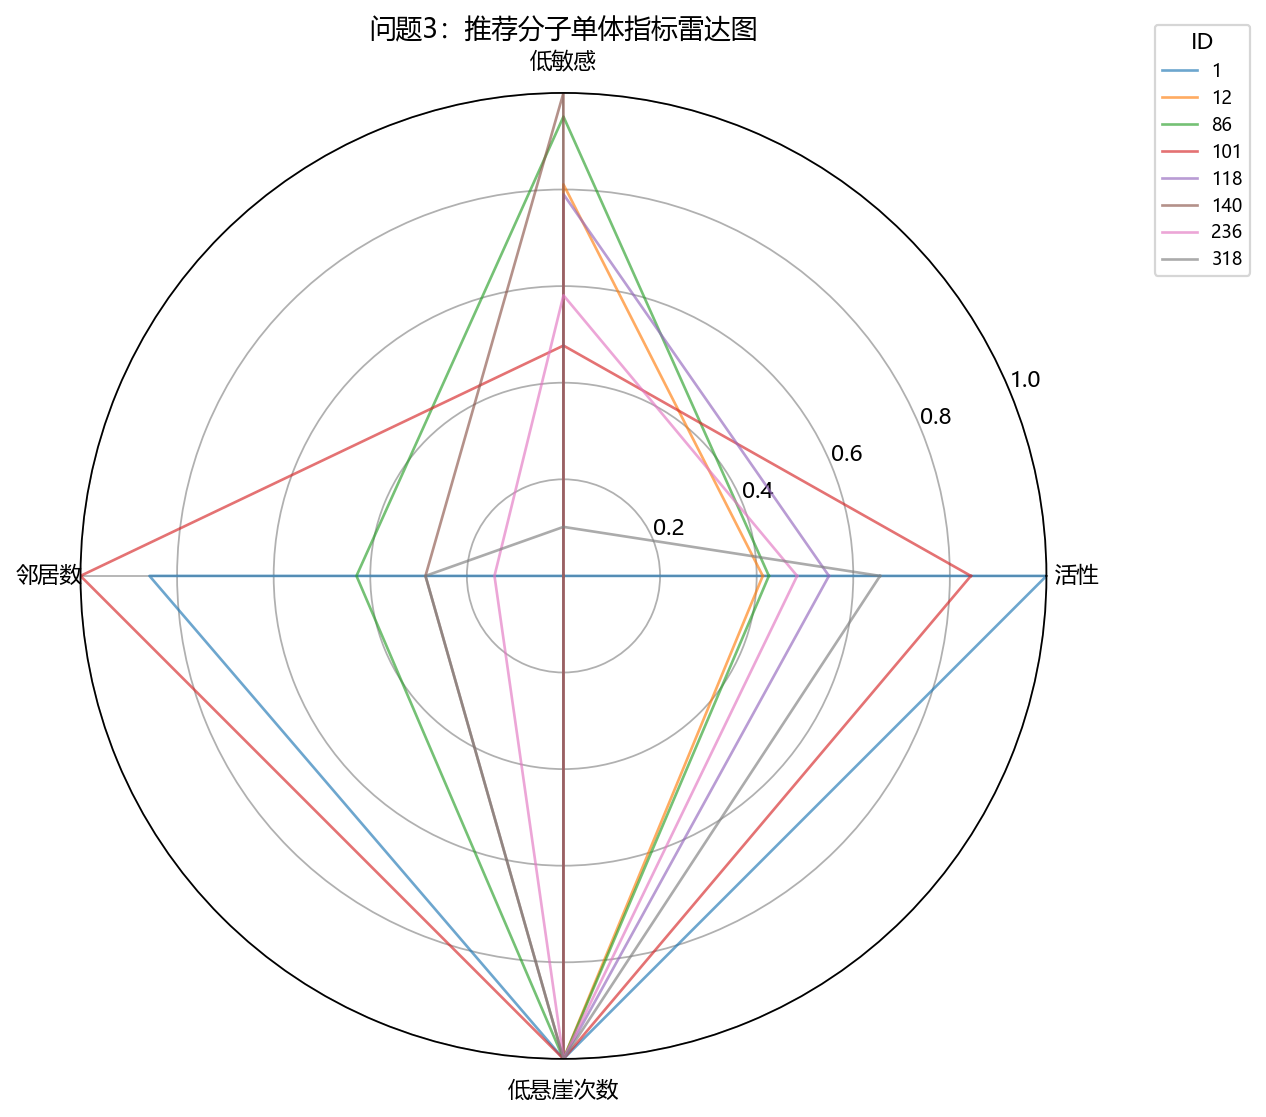
\includegraphics[width=0.82\textwidth]{问题3_推荐分子单体雷达图.png}
\caption{推荐分子的单体指标雷达图}
\end{figure}

图 12 中每条折线表示一个推荐分子，各指标均归一化到 0—1 区间。其中“活性”越大表示分子活性越高，“低敏感”越大表示局部敏感度越低，“低悬崖次数”越大表示参与活性悬崖次数越少。不同推荐分子在各指标上具有差异化特点，说明最终推荐集合不是由单一指标驱动，而是由多目标权衡形成。


\section{模型评价与改进方向}

\subsection{模型优点}

\begin{enumerate}
\item \textbf{模型解释性较强}。本文未直接套用黑箱机器学习模型，而是围绕空间邻近性、活性富集性、结构相似性和局部敏感性构建可解释指标。
\item \textbf{三问衔接自然}。第一问得到空间区域标签，第二问得到局部敏感度指标，第三问综合利用前两问结果进行实验候选分子筛选。
\item \textbf{兼顾活性与风险}。第三问没有简单选择活性最高分子，而是将活性悬崖风险纳入优选目标，更符合药物早期筛选中的稳健性需求。
\item \textbf{考虑候选集合多样性}。模型同时使用结构近邻冗余和二维空间分散度衡量多样性，避免推荐分子过度集中。

\end{enumerate}
\subsection{模型不足}

\begin{enumerate}
\item \textbf{KNN 图可能存在方向重复边}。本文在局部敏感度计算中保留有向近邻边，但若从无向分子对角度解释，后续可进一步去重分析。
\item \textbf{结构相似度信息有限}。第三问中非 KNN 近邻分子对的相似度在冗余评价中记为 0，只能表示不存在近邻冗余关系，并不代表真实结构相似度为 0。
\item \textbf{权重设置具有一定主观性}。综合评分权重体现了题目中对活性、敏感性和多样性的相对重视程度；多目标优化文献通常强调 Pareto 前沿本身不依赖权重，而单一方案选择会受到后处理偏好影响\cite{ref:ohto2026multiobjective}，因此仍可通过权重敏感性分析进一步验证推荐结果稳定性。
\item \textbf{缺少实验验证信息}。本文所有结论均基于附件数据中的活性得分、流形坐标和相似网络，实际药物发现中还需结合实验可合成性、毒性和药代动力学等信息进一步筛选。

\end{enumerate}
\subsection{改进方向}

后续可从以下方面进一步改进模型：首先，对热点区域识别中的邻域半径和活性阈值进行敏感性分析，检验分区结果稳定性；其次，在问题二中同时计算 Pearson 与 Spearman 相关系数，并对热点区域与普通区域局部敏感度差异进行显著性检验；最后，在问题三中引入权重扰动实验或鲁棒优化思想，考察最终 8 分子推荐集合对权重选择的敏感程度。


\section{结论}

本文针对 MIMAC 分子数据的活性筛选与结构风险评估问题，分别建立了高活性热点识别模型、活性悬崖与局部敏感度模型以及 8 分子多目标优选模型。

第一，基于二维流形坐标和生物活性得分，本文构建了基于活性密度的 E-DBSCAN 模型。该模型同时考虑空间邻近性和邻域活性富集程度，共识别出 12 个高活性热点区域，包含 82 个热点分子。热点区域平均活性得分为 6.2061，明显高于普通区域的 4.1201，说明模型能够有效识别高活性分子富集区域。

第二，基于 KNN 相似图和 Tanimoto 相似度，本文构建了分子对 SALI 活性悬崖指数和单分子局部敏感度指标。在 1625 条有效近邻边中，共识别出 83 对高 SALI 活性悬崖和 56 对普通活性悬崖。热点区域平均局部敏感度略高于普通区域，但中位数差异较小；活性得分与局部敏感度的 Pearson 相关系数为 0.112，说明高活性与高局部敏感度之间不存在明显强关联。

第三，本文建立了固定选取 8 个分子的多目标组合优化模型，综合考虑平均活性、平均局部敏感度、结构近邻冗余和空间分散度。通过多目标遗传算法搜索 Pareto 前沿，并用综合评分选择最终方案，推荐分子集合为

\[
\{1,12,86,101,118,140,236,318\}.
\]

该集合平均活性为 6.8153，高于全体平均水平；平均局部敏感度为 3.4643，低于全体平均水平；二维空间分散度为 16.9614，高于全体平均水平。与仅按活性排序的前 8 分子相比，本文方案在降低局部敏感风险和提高多样性方面具有明显优势，可作为下一轮实验优先验证的候选分子集合。


\begin{thebibliography}{9}
\bibitem{ref:zhao2026edbscan} 赵云龙, 孙成禹, 黄宏宇. 一种基于能量密度空间聚类算法的面波频散曲线自动拾取方法[J]. 物探与化探, 2026, 50(3): 1--9.
\bibitem{ref:guha2012landscape} Guha R. Exploring structure--activity data using the landscape paradigm[J]. \textit{WIREs Computational Molecular Science}, 2012, 2(6): 829--841.
\bibitem{ref:guha2008sali} Guha R., Van Drie J. H. The structure--activity landscape index: identifying and quantifying activity cliffs[J]. \textit{Journal of Chemical Information and Modeling}, 2008, 48(3): 646--658.
\bibitem{ref:ohto2026multiobjective} Ohto Y., Yoshikai Y., Fujimoto H., Sato K., Kusuhara H., Mizuno T. Exploring multi-objective trade-offs in reference compound selection for validation studies of toxicity assays[Z]. 2026.
\bibitem{ref:deb2002nsga2} Deb K., Pratap A., Agarwal S., Meyarivan T. A fast and elitist multiobjective genetic algorithm: NSGA-II[J]. \textit{IEEE Transactions on Evolutionary Computation}, 2002, 6(2): 182--197.
\end{thebibliography}
\begin{appendices}
\section{主要输出文件说明}

\begin{table}[H]
\centering
\caption{主要输出文件说明}
\small
\resizebox{\textwidth}{!}{%
\begin{tabular}{ll}
\toprule
文件 & 说明 \\
\midrule
\texttt{问题1\_热点区域识别结果.png} & 第一问热点区域识别可视化 \\
\texttt{问题1\_二维流形空间分子活性分布.png} & 二维流形空间活性分布图 \\
\texttt{问题1\_代表性分子.csv} & 第一问代表性分子结果 \\
\texttt{问题2\_SAS结构活性相似性图.png} & 结构—活性相似性图 \\
\texttt{问题2\_SALI活性悬崖指数分布图.png} & SALI 指数分布图 \\
\texttt{问题2\_活性得分与局部敏感度关系图.png} & 活性与局部敏感度关系图 \\
\texttt{问题3\_最终推荐8个分子.csv} & 第三问最终推荐分子结果 \\
\texttt{问题3\_推荐分子二维空间分布.png} & 推荐分子空间分布图 \\
\bottomrule
\end{tabular}%
}
\end{table}

\section{人工智能工具使用说明}

本文写作过程中使用人工智能工具辅助完成文字整理、结构润色和表达规范化。模型建立、指标含义、计算结果和结论均基于题目附件数据及已完成的数据处理结果，人工智能工具未替代数学建模过程中的数据计算与结果判断。
\end{appendices}
\end{document}
